\documentclass[a4paper,twoside]{report}
\usepackage{geometry}
\usepackage{doc}
\usepackage[latin1]{inputenc}
\usepackage[catalan]{babel}
\usepackage{amsfonts}
\usepackage{amsmath}
\usepackage[pdftex]{graphicx}
\usepackage{listings}
\usepackage{fancyhdr}
\usepackage{fancyvrb}
\usepackage{url} 
\usepackage{color}
\usepackage{lscape}
\usepackage{setspace}
\usepackage{float}
\usepackage{longtable}

\usepackage[pdfauthor={Ramon Xuriguera Albareda},%
		pdfsubject={BibTeX Bibliography Index Maker},%
		pdftitle={BibTeX Bibliography Index Maker},%
		pdftex]{hyperref}


\lstset{%
    numbers=none,               %
    breaklines=true,            %
    fancyvrb=false,             %
    tabsize=2,                  % sets default tabsize to 2 spaces
    captionpos=b,               % sets the caption-position to bottom
    frame=single,
    xleftmargin=3em,
    xrightmargin=3em,
    backgroundcolor = \color{lightgrey}
}        
\renewcommand{\lstlistingname}{Llistat}

\newcommand{\tab}{\hspace*{2em}}


\title{\BibTeX{} Bibliography Index Maker: Meeting Notes}
\author{Ramon Xuriguera}
\date{Primavera 2010}

\setlength{\parindent}{0in}
\definecolor{lightgrey}{gray}{0.85}

%%% PAGE STYLE %%%
\pagestyle{fancy}
\fancyhf{}
\renewcommand{\headrulewidth}{0pt}
\renewcommand{\footrulewidth}{0pt}
\fancyhead[LE]{\textit{\nouppercase{\leftmark}}}
\fancyhead[RO]{\textit{\nouppercase{\rightmark}}}
\fancyfoot[C]{\thepage}
 
\fancypagestyle{plain}{ %
\fancyhf{}
}

\setlength{\headheight}{14pt}


\begin{document}
\begin{titlepage}
%\thispagestyle{empty}
\vspace*{44mm}
\hspace{42mm}
\begin{minipage}{112mm}
\textbf{\textit{T�tol:} \BibTeX{} Bibliography Index Maker}\\

\textbf{\textit{Volum:} 1/1}\\
\textbf{\textit{Alumne:} Ramon Xuriguera Albareda}\\

\textbf{\textit{Director/Ponent:} Marta Arias}\\
\textbf{\textit{Departament:} LSI}\\
\textbf{\textit{Data:} Primavera 2010}\\
\end{minipage}

\end{titlepage}

\newpage
\thispagestyle{empty}
\mbox{}

\thispagestyle{empty}
\begin{doublespace}
\hrule
\vspace{5 mm}
\textbf{DADES DEL PROJECTE}
\\
\\
\textit{T�tol del Projecte:}
\\
\\
\textit{Nom de l'estudiant:} Ramon Xuriguera Albareda\\
\textit{Titulaci�:} Enginyeria Inform�tica\\
\textit{Cr�dits:} 37,5\\
\textit{Director/Ponent:} Marta Arias\\
\textit{Departament:} LSI\\
\\
\hrule
\vspace{5 mm}
\textbf{MEMBRES DEL TRIBUNAL} \textit{(nom i signatura)}\\
\\
\textit{President:}
\\
\\
\textit{Vocal:}
\\
\\
\textit{Secretari:}
\\
\\
\hrule
\vspace{5 mm}
\textbf{QUALIFICACI�}
\\
\\
\textit{Qualificaci� num�rica:}\\
\textit{Qualificaci� descriptiva:}
\\
\\
\textit{Data:}\\
\hrule
\end{doublespace}

\newpage
\thispagestyle{empty}
\mbox{}

\tableofcontents

\chapter{Introducci�}
\label{chapter:introduction}

%Aquest projecte neix amb la idea d'estalviar temps a l'hora de mantenir un cert ordre dins d'una col�lecci� de documents digitals, ja sigui per q�estions de catalogaci� o b� per poder-los citar des d'alguna altra publicaci�. 
Durant la realitzaci� d'un treball de recerca, una de les tasques a les que es dedica m�s temps �s la cerca i lectura d'articles sobre el tema que s'est� tractant. Els fitxers corresponents a aquestes publicacions habitualment es troben en format PDF \cite{isoPdf} i s'acostumen a acumular en algun directori de l'ordinador de l'investigador. Despr�s de mesos, fins i tot anys, arriba l'hora de comen�ar a escriure i �s necessari generar un �ndex bibliogr�fic d'aquests articles i aix� poder-los citar dins del nou document.

\paragraph{}
El proc�s de creaci� d'�ndexs �s repetitiu, pesat i porta molt de temps si es fa manualment. �s aqu� on entra en joc aquest projecte ja que aquesta �s una tasca que, en gran mesura, es pot automatitzar. L'objectiu principal �s el desenvolupament d'un sistema que generi autom�ticament �ndexs bibliogr�fics a partir de col�leccions de PDFs. Al llarg d'aquest document, per�, veurem que per aconseguir-ho haurem de tenir en compte altres temes interessants com poden ser l'extracci� d'informaci� estructurada i la generaci� autom�tica de regles a partir d'exemples.

\paragraph{}
Un altre aspecte a tenir en compte sobre els �ndexs �s el format que s'utilitza per crear-los, n'existeixen molt�ssims. En disciplines de caire cient�fic i t�cnic com ara les matem�tiques, f�sica o inform�tica, l'eina est�ndard usada per escriure articles �s \LaTeX{}, i normalment es complementa amb el gestor bibliogr�fic \BibTeX{}. �s per aix� que s'ha optat per aquest format i, de fet, �s el que d�na nom al projecte.


%En principi, aix� pot interessar a qualsevol persona que hagi de redactar un text i necessiti portar un control de tots els altres documents als quals es refereix. De totes maneres, el punt de vista que s'ha adoptat �s una mica m�s restringit, semblant al que poden tenir els membres de la comunitat cient�fica a l'hora d'escriure articles, ja que ens aprofitarem d'algunes de les peculiaritats d'aquest tipus d'escrits. 

%1. Proces t�pic a l'hora de fer un treball de recerca: primer, llegir sobre el tema (literature review), despres treballar sobre el tema i continuarllegint, guardant els articles rellevants en una carpeta, molt probablement en format PDF. Aix� durant possiblement mesos o fins i tot anys! (gran quantitat d'articles en PDF!!)

%2. Quan ja es vol comen�ar a escriure, s'ha de fer un index bibliogr�fic a partir dels articles que s'han anat recopilant. Proces pesat i "time-consuming".

%3. Aix� �s el que aquest projecte vol fer: estalviar a l'investigador aquesta feina, en gran mida automatitzable, de generar un index bibliogr�fic per la seva refer�ncia a partir de les col.leccions de pdfs.

%4. Est�ndar a l'inform�tica i mates i altres disciplines d'enginyeria i t�cniques: latex i bibtex. Per aix� s'ha optat per fer l'index en bibtex.

%I, de fet, pots seguir amb la descripci� de les eines disponibles que faciliten la gesti� de refer�ncies per posar de manifest que aquesta funcionalitat no existeix.




\paragraph{}
El problema que acabem de descriure no �s nou i existeix un gran nombre d'eines destinades a facilitar la gesti� de refer�ncies o b� a oferir altres serveis relacionats. Totes les que coneixem es poden classificar en alguna d'aquestes tres categories:
\begin{itemize}
\item{}
%\paragraph{}
En primer lloc, hi ha el que s'anomenen \textit{biblioteques digitals}, grans bases de dades amb informaci� sobre articles, els seus autors i, en alguns casos, tamb� sobre les relacions de citaci� entre ells. Estan disponibles en l�nia i tothom pot consultar-les. Alguns exemples s�n \textit{DBLP} o b� \textit{RePEc}.
\item{}
%\paragraph{}
Despr�s, tenim nombroses aplicacions dedicades al maneig de refer�ncies com ara \textit{JabRef} \cite{JabRef} o \textit{Mendeley}\cite{Mendeley}. Algunes d'aquestes eines inclouen funcionalitats no tant relacionades amb la gesti� sin� amb l'obtenci� de refer�ncies. Per exemple, n'hi ha que ofereixen la possibilitat de cercar en les biblioteques esmentades al punt anterior. Altres, permeten obtenir informaci� continguda dins de les meta-dades dels fitxers. A part d'aix�, no hem trobat cap eina que aprofiti el contingut dels documents per generar la refer�ncia.

\item{}
%\paragraph{}
Finalment, tamb� existeixen serveis com ara \textit{Google Scholar}, \textit{Microsoft Academic Search} o \textit{CiteSeer} que es dediquen a recol�lectar i indexar informaci� sobre articles i que comptabilitzen les refer�ncies entre diferents publicacions. En el cas de \textit{CiteSeer}, al ser un projecte lliure, sabem que funciona analitzant les diferents parts dels articles, com ara les cites, per� que t� problemes per obtenir els camps de la cap�alera \cite{Giles98citeseer}.
\end{itemize}

\paragraph{}
El sistema que resulta d'aquest projecte mira d'unir, de cara a l'usuari, aquests tres tipus de programari: primer, genera refer�ncies recolzant-se a les biblioteques digitals i cercadors; un cop generades, poden ser importades i gestionades amb les eines de maneig descrites al segon punt. 

%%%% ESTRUCTURA DOCUMENT %%%%
\section{Sobre aquest document}
La mem�ria est� dividida en els cap�tols seg�ents:

\begin{itemize}
\item{Cap�tol \ref{chapter:definition}:}
Descripci� formal del projecte aix� com un breu rep�s sobre el disseny i implementaci�.

\item{Cap�tol \ref{chapter:search}:}
Parla de les t�cniques que s'utilitzen per poder aconseguir p�gines que continguin informaci� sobre els documents pels quals es volen obtenir refer�ncies.

\item{Cap�tol \ref{chapter:refextraction}:}
Tracta de com ho fem per extreure la informaci� sobre els articles de les p�gines d'Internet que hem obtingut al tercer cap�tol.

\item{Cap�tol \ref{chapter:wrapperinduction}:}
Est� dedicat a les t�cniques per generar, de forma autom�tica, les regles d'extracci� de les refer�ncies.

\item{Cap�tol \ref{chapter:results}:}
Plantejament de les proves per cadascuna de les parts m�s importants del sistema i an�lisi dels resultats obtinguts.
\end{itemize}

Respecte al contingut de les diferents seccions, hem provat de centrar-nos, sobretot, en les decisions que hem hagut de prendre al llarg de la realitzaci� del projecte; indicant-ne algunes de les opcions plantejades en un principi, els problemes que aquestes presenten i la descripci� de la soluci� escollida finalment. S'han intentat ometre molts dels aspectes m�s t�cnics sobre la implementaci� del sistema, aix� com definicions i descripcions detallades de les tecnologies utilitzades.

\paragraph{}
S'assumeix que es tenen nocions b�siques sobre l'estructura dels documents HTML i sobre expressions regulars, dos temes que no es tractaran. Pel que fa a les expressions regulars, cal assenyalar que s'utilitzen les operacions que ofereix el m�dul \texttt{re} de \textit{Python}. Es pot trobar m�s informaci� a \cite{pyRegex}.


\chapter{Definici� del Projecte}
\label{chapter:definition}


%%%% FUNCIONALITATS %%%%
\section{Requeriments}
A continuaci� es llisten totes les funcionalitats que l'aplicaci� haur� d'oferir a l'usuari. Cal comentar que aquests requeriments els hem establert nosaltres mateixos a segons el que ens ha semblat m�s necessari.
\begin{itemize}
\item{}
Extracci� de la refer�ncia bibliogr�fica corresponent a un o m�s articles que es troben en fitxers PDF dins d'algun directori.

\item{}
Possibilitat d'exportar les refer�ncies extretes en el format \BibTeX{} i desar-les a un fitxer \texttt{.bib}

\item{}
Generaci� autom�tica de regles d'extracci� a partir d'exemples.

\item{}
Importaci� de refer�ncies en un fitxer \texttt{.bib} per tal de poder-los fer servir d'exemples.

\item{}
Totes les operacions CRUD\footnote{\textit{Create}, \textit{read}, \textit{update} i \textit{delete}.} per a la gesti� de refer�ncies i regles d'extracci�.
\end{itemize}


\section{L'extracci� de refer�ncies}
Aquest �s l'objectiu principal de l'aplicaci� i les limitacions que hem trobat per aconseguir-lo s�n les que han guiat el disseny de la resta del sistema. A continuaci� es pret�n mostrar, a grans trets, el raonament seguit a l'hora de definir una estrat�gia amb certes garanties d'�xit. En un principi, la idea que vam plantejar per resoldre el problema de l'extracci� de refer�ncies d'un document PDF era intentar agafar la informaci� de la refer�ncia bibliogr�fica directament del fitxer, seguint uns passos semblants als de la figura seg�ent.

\begin{figure}[H]
\begin{center}
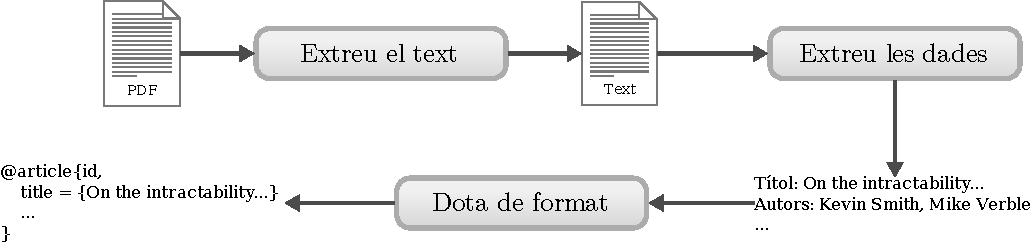
\includegraphics[width=\textwidth]{figures/definition:invalid-extraction-diagram.pdf}
\caption{Primera idea per l'extracci� de refer�ncies}
\label{fig:definition:invalid-extraction-diagram}
\end{center}
\end{figure}

Aix� presenta moltes limitacions. Per comen�ar, hi ha la impossibilitat d'extreure informaci� que no es troba dins del text (e.g. el n�mero de p�gines de l'article). Una altra �s que la informaci� dins dels fitxers PDF no t� una estructura prou clara com per poder distingir entre els diferents camp. Aquest segon problema es tracta amb m�s en detall al proper cap�tol.

\paragraph{}
La soluci� que hem trobat per poder tirar endavant consisteix en fer �s de les biblioteques digitals descrites a la introducci�. La majoria d'elles estan indexades pels principals cercadors disponibles a Internet. El diagrama actualitzat es mostra a la figura \ref{fig:definition:extraction-diagram}. B�sicament, per cada fitxer l'aplicaci�:
\begin{enumerate}
    \item{Extreu el contingut en forma de text.}
    \item{Genera un llistat de consultes a partir del text extret.}
    \item{Obt� els resultats d'aquestes consultes amb algun cercador (Google, Bing, etc.).}
    \item{Mira d'extreure la refer�ncia de les p�gines retornades pel cercador.}
    \item{Comprova que les dades de la refer�ncia realment corresponguin a l'article contingut pel fitxer.}
    \item{D�na format a les dades de la refer�ncia.}
\end{enumerate}

\begin{figure}[H]
\begin{center}
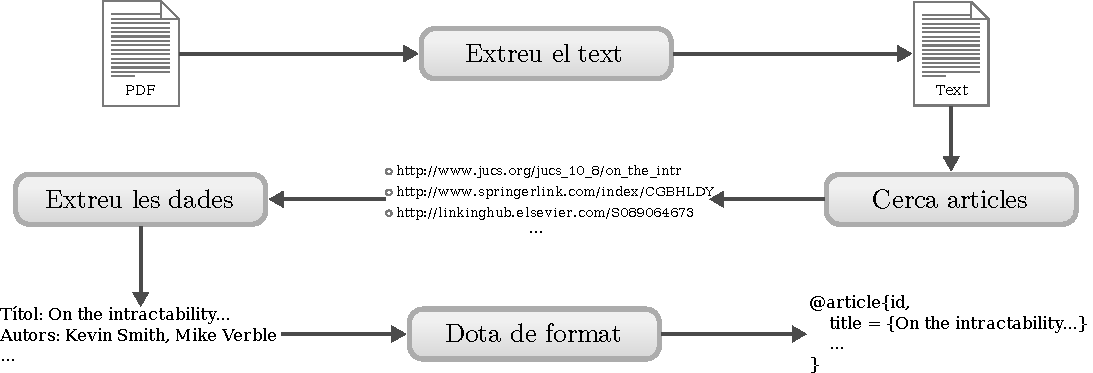
\includegraphics[width=\textwidth]{figures/definition:extraction-diagram.pdf}
\caption{Esquema del proc�s a seguir per extreure una refer�ncia}
\label{fig:definition:extraction-diagram}
\end{center}
\end{figure}

El motiu que fa que aquest procediment es pugui implementar en el temps del que disposem �s que les dades ofertes per les biblioteques digitals en els documents HTML est� molt estructurada. Com �s l�gic, tenen la informaci� emmagatzemada en bases de dades, i a l'hora de mostrar-la als usuaris, la formaten de manera autom�tica; sempre de la mateixa manera (amb algunes excepcions). Aquesta estructura fixa al llarg de les p�gines d'una mateixa biblioteca �s el que realment simplifica la tasca d'extracci�, ja permet generar regles que funcionin en un percentatge molt alt dels casos.

\paragraph{}
Aix� doncs, hem de fer una mica m�s de tomb per poder aconseguir els resultats desitjats, per� els passos s�n m�s senzills d'aplicar. El problema que ten�em al principi ha quedat dividit en tres problemes m�s petits:
\begin{itemize}
\item{}
La cerca de les p�gines amb informaci� de l'article.
\item{}
Extracci� de la refer�ncia d'aquestes p�gines.
\item{}
Generaci� de les regles d'extracci�. (Les anomenarem \textit{wrappers})
\end{itemize}
Cadascuna d'aquestes parts es tracta per separat en els propers cap�tols.

%%%% BIBTEX %%%%
\section{\BibTeX}
\label{chapter:definition:section:bibtex}
Per poder entendre el context del projecte cal que descrivim l'eina de maneig de refer�ncies \BibTeX{} i la sintaxi del llenguatge que utilitza. 
En el nostre cas farem servir aquest llenguatge com a format de sortida al generar els �ndexos bibliogr�fics. Al llistat \ref{listing:exampleBibTeX} es mostra un exemple d'una refer�ncia d'un article cient�fic expressat en el format \BibTeX:
\begin{center}
\begin{lstlisting}[caption={Refer�ncia expressada en \BibTeX}, label=listing:exampleBibTeX]
@article{MoSh:27,
  title = {Size direction games over the real line},
  author = {Moran, Gadi and Shelah, M., Saharon},
  journal = {Israel Journal of Mathematics},
  pages = {442--449},
  volume = {14},
  year = {1973},
}
\end{lstlisting}
\end{center}

Alguns aspectes a comentar sobre l'exemple anterior:
\begin{itemize}
\item{}
La primera l�nia cont� el tipus de document i un identificador. El primer defineix els camps obligatoris que s'han d'especificar, i el segon ens permetr� citar a la refer�ncia des d'un document. En el nostre cas nom�s ens interessen les refer�ncies de tipus \textit{article} i haurem de definir, com a m�nim, els camps \textit{author}, \textit{title}, \textit{journal} i \textit{year}, que s�n obligatoris.

\item{}
Es considera que el nom d'un autor o editor pot constar de quatre parts diferents: \textit{First}, \textit{von}, \textit{Last}, \textit{Jr.}. Es poden ordenar de diverses maneres, per� nosaltres ho farem amb \texttt{<von> <last>, <middle>, <first>}. Cal separar m�ltiples noms amb la paraula \texttt{and}.

\item{}
L'�ltim camp d'una refer�ncia pot acabar o no amb una coma.
\end{itemize}




\section{Disseny del sistema}
Hem estructurat el codi en diferents m�duls independents; es llisten a continuaci�:
\begin{itemize}
\item{\textit{Raw Content Extraction} (\texttt{rce}):}
Agrupa totes les classes encarregades d'extreure el contingut dels documents PDF.

\item{\textit{Information Retrieval} (\texttt{ir}):}
Encarregat de comunicar-se amb els diferents cercadors suportats per obtenir p�gines que contenen informaci� de la refer�ncia que volem extreure.

\item{\textit{Information Extraction} (\texttt{ie}):}
Cont� tot el codi que permet obtenir la refer�ncia a partir d'una p�gina HTML. A m�s, tamb� �s l'encarregat de generar nous \textit{wrappers}.

\item{\textit{References} (\texttt{references}):}
Per una banda fa un an�lisis sint�ctic de les refer�ncies extretes per poder-les validar. Per l'altra, les transforma a \BibTeX{}.

\item{Base de dades (\texttt{db}):}
Tal i com indica el seu nom, duu a terme els accessos la base de dades.

\item{\textit{Main} (\texttt{main}): }
Enlla�a tots els m�duls anteriors i proporciona punts d'entrada a la interf�cie d'usuari. Fa de fa�ana del sistema.

\item{\textit{Graphical User Interface} (\texttt{ui}):}
Interf�cie d'usuari m�s o menys amigable.
\end{itemize}

La figura \ref{fig:module_diagram} mostra com interaccionen entre ells. Els m�duls que s'encarreguen de les operacions m�s b�siques s�n independents entre ells. El m�dul \textit{main} utilitza aquestes operacions per definir el flux de la informaci� i ofereix serveis a la capa superior: la interf�cie d'usuari.

\begin{figure}[H]
\begin{center}
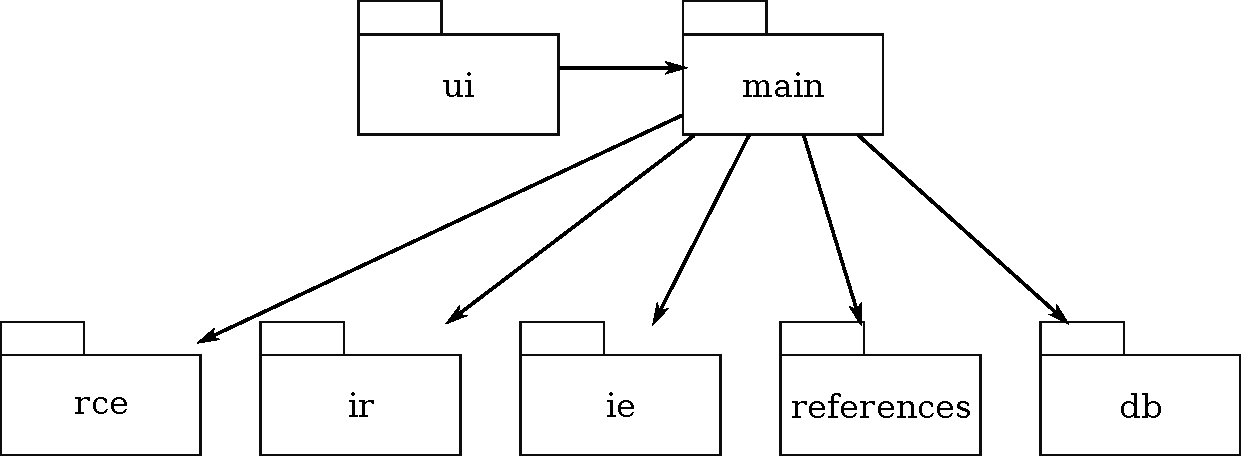
\includegraphics[width=0.7\textwidth]{figures/module_diagram.pdf}
\caption{M�duls del sistema}
\label{fig:module_diagram}
\end{center}
\end{figure}


%%%% LLIC�NCIA %%%%
\section{Llic�ncia}
L'aplicaci� es distribueix sota  una lic�ncia lliure que permet als destinataris la possibilitat de copiar, modificar i redistribuir el codi. Concretament, hem escollit la \textit{General Public License} (GPL) v.3, que requereix que qualsevol treball derivat tamb� es distribueixi amb els mateixos permisos. El text complet d'aquesta llic�ncia es pot trobar a \cite{gpl3} aix� com al fitxer \texttt{LICENSE} que acompanya al codi.

\paragraph{}
Qualsevol interessat pot agafar el codi i modificar-lo tan per afegir noves funcionalitats com per arreglar errors. La forma m�s f�cil de fer-ho �s anar al repositori on es troba el projecte (\cite{repo}) i fer un \textit{fork}. D'aquesta manera, el nou codi sempre es podr� fusionar a la branca \textit{oficial}.

\section{Llista de tasques}
A continuaci� s'esmenten les tasques m�s importants que s'han dut a terme i elements que s'han implementat durant la realitzaci� del projecte. S'acompanyen amb una estimaci� del temps que ha estat necessari per completar-les, per donar una idea del pes de cadascuna d'elles:

\begin{center}
\begin{longtable}{|l r|}

\hline
\textbf{Tasca}                                                              & \textbf{Temps estimat}\\
\hline
\hline
Recerca i proves de concepte                                                & \textbf{20 dies}\\
\hline
Configuraci� de la infraestructura                                          & \textbf{4 dies}\\
\tab Repositori (\textit{GitHub}): Creaci� i estructura del projecte        & 1 dia\\
\tab \textit{Build tracker}                                                 & 3 dies\\   
\hline                                                                            
Extracci� del text dels PDF (\texttt{bibim.rce})                            & \textbf{8 dies}\\
\tab Cerca d'eines i comparaci� de resultats                                & 5 dies\\
\tab Codi de l'extracci�                                                    & 3 dies\\
\hline                                                                            
Obtenci� de p�gines amb la refer�ncia (\texttt{bibim.ir})                   & \textbf{13.5 dies}\\
\tab Proves amb diferents cercadors i \textit{XGoogle} (veure l'ap�ndix \ref{appendix:libraries:xgoogle})                     & 4 dies\\
\tab Obtenir consultes del text                                             & 1.5 dies\\
\tab \textit{Browser} per obtenir p�gines de la Web                         & 2 dies\\
\tab Codi per la cerca de les consultes                                     & 5 dies\\
\tab Ordenaci� resultats de la cerca                                        & 1 dia\\   
\hline                                                                            
Extracci� d'informaci� (\texttt{bibim.ie})                                  & \textbf{14 dies}\\
\tab An�lisi de l'estructura d'algunes biblioteques digitals disponibles    & 5 dies\\
\tab Regles a m� per extreure refer�ncies directament                       & 3 dies\\
\tab Regles a m� per extreure camps                                         & 2 dies\\                    
\tab Validaci� de les refer�ncies extretes                                  & 4 dies\\
\hline                                                                            
Generaci� autom�tica de \textit{wrappers} (\texttt{bibim.ie})               & \textbf{32.5 dies}\\
\tab Extracci� d'exemples                                                   & 1.5 dies\\
\tab Validaci� dels exemples extrets                                        & 0.5 dies\\
\tab \textit{Wrapper} gen�ric                                               & 0.5 dies\\
\tab Generaci� autom�tica de regles                                         & 27 dies\\
\tab \tab Camps de valor �nic                                               & 17 dies\\
\tab \tab Camps multi valor                                                 & 10 dies\\
\tab Avaluaci� de les regles generades                                      & 3 dies\\
\hline                                                                            
Tractament de refer�ncies (\texttt{bibim.references})                       & \textbf{5 dies}\\
\tab \textit{Parsing}                                                       & 2 dies\\
\tab Generaci� i Format                                                     & 2 dies\\
\tab Creaci� �ndexs                                                         & 1 dia\\
\hline                                                                            
Base de dades (\texttt{bibim.db})                                           & \textbf{5 dies}\\
\tab Disseny                                                                & 1 dia\\
\tab \textit{Mappers} amb SQLAlchemy                                        & 4 dies\\    
\hline                                                                            
M�dul principal (\texttt{bibim.main})                                       & \textbf{11 dies}\\
\tab Escaneig de fitxers                                                    & 1 dia\\
\tab \textit{Threading}                                                     & 2 dies\\
\tab Comunicaci� dels m�duls anteriors                                      & 8 dies\\
\hline                                                                            
Interf�cie d'usuari (\texttt{bibim.ui})                                     & \textbf{4 dies}\\
\tab Editor de refer�ncies                                                  & 1.5 dies\\
\tab Editor de \textit{wrappers}                                            & 1 dia\\
\tab Resta de vistes                                                        & 1.5 dies\\ 
\hline
Proves                                                                      & \textbf{12 dies}\\
\tab Col�leccionar PDF, HTML i \BibTeX{} de mostra                          & 3 dies\\
\tab \textit{Scripts} per automatitzar                                      & 6 dies\\
\tab Execuci� i an�lisi de resultats                                        & 3 dies\\
\hline
\hline
\end{longtable}
\end{center}

\chapter{Cerca de refer�ncies}
\label{chapter:search}

%%%% EXTRACCI� PDF %%%%
\section{Extracci� dels continguts d'un PDF}
El primer pas per poder obtenir la refer�ncia d'un article en un fitxer PDF �s l'extracci� del contingut d'aquest fitxer. Aquest �s un dels aspectes que han influ�t m�s en l'enfocament que hem donat al sistema, pels motius que es descriuen a continuaci�.
\paragraph{}
Tal i com ja hem esmentat, en un principi, la soluci� que es va plantejar era intentar extreure la refer�ncia bibliogr�fica d'un document directament del fitxer PDF del qual es disposa. Tot i les limitacions que aix� suposa, despr�s de veure com queden els articles al convertir-los a text ens vam allunyar encara m�s d'aquesta idea.
\\

\begin{lstlisting}[caption={Text corresponent a la cap�alera d'un article despr�s d'haver-lo extret d'un PDF}, label=listing:examplePDFExtraction01]
Characterization and Armstrong Relations for Degenerate Multivalued Dependencies Using Formal Concept Analysis
Jaume Baixeries and Jos� Luis Balc�zar e a
Dept. Llenguatges i Sistemes Inform`tics, a Universitat Polit`cnica de Catalunya, e c/ Jordi Girona, 1-3, 08034 Barcelona {jbaixer, balqui}@lsi.upc.es

Abstract. Functional dependencies, a notion originated ...
\end{lstlisting}

Els llistats \ref{listing:examplePDFExtraction01} i \ref{listing:examplePDFExtraction02} mostren exemples de les cap�aleres de dos articles diferents despr�s d'haver extret el text del fitxer PDF en el que es trobaven. Com es pot veure, el resultat no t� cap tipus d'estructura que pugui deixar intuir quina part del text correspon a cada fragment d'informaci�, sin� que �s un conglomerat de totes dades. El primer article comen�a amb el t�tol i segueix amb els noms dels dos autors i la informaci� de la universitat. En canvi, el segon comen�a amb l'any, la confer�ncia on s'ha presentat, t�tol i per cada autor es d�na informaci� diferent sobre la universitat. Si comencem a mirar m�s articles, el n�mero de casos amb estructures diferents no para d'augmentar (hi ha m�s exemples a l'ap�ndix \ref{appendix-pdf2text}).
\\

\begin{lstlisting}[caption={Un altre exemple de text extret d'un PDF}, label=listing:examplePDFExtraction02]
2010 Second International Conference on Future Networks

Cloud Computing Research and Development Trend
Shuai Zhang Hebei Polytechnic University College of Science Hebei Polytechnic University NO.46 Xinhua West Street Tangshan 063009, Hebei Province China zhangshuai@heut.edu.cn Xuebin Chen Hebei Polytechnic University College of Science Hebei Polytechnic University NO.46 Xinhua West Street Tangshan 063009, Hebei Province China chxb@qq.comm
Abstract--With the development of parallel computing, distributed [...]
\end{lstlisting}

Una vegada vistos els resultats, probablement queda m�s clara la inviabilitat de la primera opci� i per qu� hem decidit consultar la informaci� dels articles que hi ha disponible a la xarxa. De totes maneres, continua sent necess�ria l'extracci� del text dels PDFs per tal de poder fer cerques, i cal veure com ho podem fer.

%%%% DIFICULTATS %%%%
\subsection{Dificultats}
Tot hi haver-hi diverses utilitats que permeten l'extracci� del contingut d'un fitxer PDF en forma de text pla o HTML, totes presenten problemes similars als de la llista seg�ent:
\begin{itemize}
\item{No extreuen b� els car�cters especials com ara Unicode o lligadures (e.g. \textit{fi} es representa com un sol car�cter)} 

\item{Sub/Super�ndexs:}
la majoria d'eines els extreuen com text que forma part de la paraula. Per exemple: \textit{Joan$^{3}$} s'extreu com a \textit{Joan3}

\item{Flux del text dins del fitxer:}
Hi ha casos en que el text es troba en diferents columnes i a l'hora d'agafar-lo, aquestes columnes o seccions no han d'estar mesclades.

\item{Fragmentaci� de par�grafs:}
Relacionat amb el punt anterior. Hi ha ocasions on els par�grafs es divideixen en un conjunt de l�nies segons com es troben posicionades dins del document. El text resultant cont� salts de l�nia addicionals que s'han introdu�t per conservar les mateixes l�nies del document original, sense tenir en compte l'estructura l�gica.
\item{Fitxers protegits dels quals no es pot extreure el contingut}
\end{itemize}

\paragraph{}
Una altra situaci� en que no serem capa�os d'extreure el text del PDF �s en aquells casos que els fitxers enlloc de contenir text, contenen imatges amb el document escanejat i no han estat processats per cap programari de reconeixement de car�cters. Pel que hem vist, aix� sol passar sobretot per articles de fa uns quants anys.

%%%% PROGRAMARI %%%%
\subsection{Programari}
El llistat de programari lliure disponible per a dur a terme l'extracci� del contingut �s for�a redu�t i totes presenten alguns dels problemes (o tots) que acabem de comentar. Tot i aix�, hem tingut en compte diverses opcions abans d'escollir una biblioteca o aplicaci� d'extracci�. Hem contemplat: \textit{PyPDF}, \textit{PDFMiner}, \textit{PDFBox}, per� finalment ens hem decantat per \textit{xPDF}.

\paragraph{}
\textit{xPDF} consisteix en un conjunt d'eines executables des de la l�nia de comandes que permeten extreure text i altres elements dels fitxers PDF. Es distribueixen sota la llic�ncia GPL v.2 i hi ha binaris tant per Windows com per Linux (que tamb� funcionen per Mac OS). El motiu principal pel qual hem escollit aquesta eina �s que s'obtenen resultats relativament bons. En especial, �s interessant el fet que no separa els par�grafs en diferents l�nies i que en la majoria dels casos respecta el flux del text dins del document. 

\paragraph{}
Pel que fa als car�cters especials, transforma b� les lligadures en m�ltiples car�cters, per� t� problemes amb la codificaci� Unicode. Donat que la majoria dels articles cient�fics estan escrits en angl�s, aquest �s un problema que hem decidit obviar. Tal i com veurem, a no ser que l'article contingui un percentatge molt elevat d'aquest tipus de car�cters, ser� igualment possible extreure'n la refer�ncia.

%%%% CONSULTES %%%%
 \section{Consultes}
 \label{section:chapter-search:consultes}
El m�s important per poder cercar refer�ncies bibliogr�fiques a Internet �s ser capa�os de generar consultes que retornin bons resultats. Per fer-ho, agafarem porcions del text extret amb l'eina \textit{xPDF} i les utilitzarem per obtenir resultats que hi coincideixin exactament. 

\paragraph{}
Una primera idea pot consistir a cercar segons el t�tol de la publicaci� de la qual volem informaci�. El problema �s que bona part dels resultats corresponen a p�gines que fan refer�ncia a aquesta publicaci�, per� que no en donen gaires detalls. Agafant la resta d'informaci� de la cap�alera (e.g. autors, revista) les consultes encara seran menys restrictives i retornaran resultats pitjors. Per una altra banda, si intentem fer consultes a partir del contingut del mateix article ens trobem amb que en molts casos, els cercadors no el tenen indexat. 

\paragraph{}
Una tercera opci�, que �s la que utilitzem, consisteix a generar les consultes del resum o \textit{abstract} que acompanya la majoria d'articles i que tamb� acostuma a apar�ixer a les p�gines que contenen la refer�ncia. Per� com podem saber quina part del text que hem extret correspon al resum? Tot i que en moltes vegades el primer par�graf va precedit de la paraula \textit{Abstract}, tamb� n'hi ha moltes altres en que va precedit d'una paraula completament diferent (e.g. resum o \textit{summary}) o b� per cap. Per tal que el sistema sigui el m�s general possible, enlloc de fixar-nos en paraules concretes fem servir una expressi� regular molt simple que permet trobar cadenes amb un n�mero de paraules determinat. 

\paragraph{}
Un dels trets caracter�stics de les cap�aleres dels articles una vegada n'hem extret el text �s que contenen un nombre elevat de s�mbols especials. Aix� ens pot ajudar a distingir entre les parts corresponents a la cap�alera i el resum. L'expressi� regular que obt� les consultes �s: \verb=([\w()?!]+[ ]){min,max}= i agafar� seq��ncies de \textit{min} a \textit{max} paraules separades per un espai i formades per car�cters alfanum�rics i un nombre limitat de s�mbols. Els par�metres \textit{min} i \textit{max} s�n configurables. �bviament, les consultes que ens d�na aquesta expressi� no sempre s�n bones i per tal de contrarestar aquests errors, en generem v�ries i les anem utilitzant mentre no s'obtinguin resultats satisfactoris. De totes maneres, tal i com es pot veure al cap�tol \ref{chapter:results}, no �s necessari ni generar moltes consultes ni cal que aquestes siguin gaire llargues.

\paragraph{}
A continuaci� es llisten cinc consultes extretes d'un article d'exemple. Noteu que s'envolten de cometes dobles, la forma habitual d'indicar als cercadors que les coincid�ncies han de ser exactes.
\begin{itemize}
\item{``are known to admit interesting characterizations in terms of Formal''}
\item{``natural extensions of the notion of functional dependency are the''}
\item{``We propose here a new Galois''}
\item{``which gives rise to a formal concept lattice corresponding precisely''}
\item{``the degenerate multivalued dependencies that hold in the relation''}
\end{itemize}

\paragraph{}
\label{chapter:search:skip-queries}
En molts casos, l'expressi� regular anterior tamb� d�na coincid�ncies pel t�tol de l'article. Per evitar el problema que hem descrit, hi ha definit un altre par�metre que estableix el nombre de consultes a saltar-se des del principi de l'article. �s una manera rudiment�ria d'aconseguir-ho, per� funciona la majoria de vegades.



%%%% CERCADORS %%%%
\section{Cercadors}
\label{section:search:searchers}
El seg�ent pas despr�s d'haver obtingut un conjunt de consultes �s utilitzar-les amb un cercador per tal d'obtenir p�gines amb informaci� de la refer�ncia que volem aconseguir. Al cap�tol d'introducci�, hem esmentat que hi ha cercadors com ara \textit{Google Scholar} o \textit{Microsoft Academic Search} on els resultats nom�s corresponen a publicacions. En un principi ens va semblar raonable intentar fer �s d'aquests serveis per poder aconseguir els nostres objectius. El problema �s que no tenen cap API publicada que permeti fer consultes autom�tiques des d'aplicacions de tercers. Tot i que hi ha solucions i \textit{workarounds}, van en contra dels termes i condicions i els servidors bloquegen massa consultes seguides. Per tant, hem descartat aquesta opci�.

\paragraph{}
Aix� doncs, ens quedem amb els cercadors de prop�sit general; hem preparat la nostra aplicaci� per tal d'utilitzar les APIs de \textit{Google}, \textit{Yahoo} i \textit{Bing}. Tots tres cercadors retornen els resultats en format JSON. Els principals inconvenients s�n que retornen qualsevol tipus de p�gina i que no tenen indexades algunes biblioteques digitals, per� en general, podem aconseguir bons resultats amb l'�s de les consultes adequades. Al cap�tol de resultats (\ref{chapter:results:section:search}) hi ha una comparativa.


%%%% ORDENACI� RESULTATS %%%%
\subsection{Ordenaci� de resultats}
La majoria de vegades, no ens convindr� l'ordre dels resultats donat pels diferents cercadors sin� que voldrem processar les p�gines segons aquelles per les quals tenim regles d'extracci�. �s per aix� que un cop hem consultat al cercador, comprovem si tenim regles per alguna de les p�gines resultants i, en cas afirmatiu, la movem a dalt de tot de la llista. 

\paragraph{}
Fem �s d'una cua de prioritats a l'hora de fer l'ordenaci�, aix� podem establir, segons la qualitat de les regles, quines s'han de provar primer. Un dels factors que intervenen per establir la \textit{qualitat}, �s una puntuaci� que s'assigna a les regles de les que disposem. Aquest tema de les puntuacions es tracta amb m�s detall al cap�tol sobre generaci� de \textit{wrappers} (\ref{chapter:wrapperinduction}). 


%%%% AJUSTAMENTS %%%%
\subsection{Altres Ajustaments}
Depenent de l'estructura del contingut dels fitxers dels que disposem, la qualitat dels resultats obtinguts amb els cercadors pot variar considerablement. Aix� suposa la necessitat d'ajustar alguns par�metres per tal de poder adaptar el sistema a l'�s de cadasc�. A la secci� sobre la generaci� de consultes (\ref{section:chapter-search:consultes}), ja hem comentat la possibilitat d'ajustar el m�nim i m�xim de termes a cercar, per� hi ha altres opcions que es poden configurar.

\paragraph{}
En algunes ocasions, es d�na el cas que la consulta generada no �s prou restrictiva, ja sigui perqu� no �s prou llarga o b� perqu� est� formada per paraules molt generals. Al cercar amb aquestes consultes s'obt� una llarga llista de resultats, la majoria dels quals no tenen res a veure amb la informaci� que estem buscant. Per contrarestar-ho, hi ha la possibilitat d'indicar al sistema que ometi els resultats i provi amb la seg�ent consulta. A l'hora d'assignar el valor d'aquest par�metre, tamb� s'haur� de tenir en compte el tipus d'articles dels que es vol informaci�. Per exemple, els articles populars segurament tindran un n�mero de coincid�ncies rellevants gran i, per tant, haurem d'assignar un valor relativament alt, ja que un valor baix far� que descartem resultats bons. En canvi, per articles poc corrents, ens interessar� el contrari.

\paragraph{}
Per una altra banda,  hi ha ocasions en que els cercadors tenen tend�ncia a retornar resultats que, tot i coincidir amb la consulta que li hem donat, corresponen a una p�gina que no ens aporta massa informaci�. Per tal d'ajudar a l'aplicaci� a descartar resultats dolents, podem indicar-li p�gines que volem ometre a partir d'una llista negra. Per exemple, sabem que les p�gines sobre els autors de la biblioteca digital \textit{ACM Portal} contenen un llistat de tots els articles d'un mateix autor, per� que no contenen suficient informaci� com per extreure refer�ncies. En aquest cas voldrem descartar els resultats que comencen per \href{http://portal.acm.org/author\_page.cfm?id=}{http://portal.acm.org/author\_page.cfm}.

\section{\textit{Multithreading}}
Un dels inconvenients m�s grans que implica el fet d'haver d'accedir a Internet, �s que el temps perdut esperant dades �s molt alt. Per reduir-lo, s'ha estudiat la possibilitat d'utilitzar diferents fils d'execuci� per fer m�s d'una consulta de forma m�s o menys simult�nia. La taula seg�ent mostra una comparativa del temps necessari per obtenir m�tliples p�gines web de forma seq�encial o b� utilitzant fins a cinc fils d'execuci� diferents. Les p�gines corresponen a consultes aleat�ries a \textit{Google} per evitar l'efecte dels \textit{proxies} i \textit{caches}. 

    \begin{center}
    \begin{tabular}{|r|r||r|r||r|r||r|r|}
        \hline
        \multicolumn{2}{|c||}{2 p�gines} & \multicolumn{2}{|c||}{5 p�gines} & \multicolumn{2}{|c||}{10 p�gines} & \multicolumn{2}{|c|}{20 p�gines} \\
        \hline
        Seq. & 5 Threads          & Seq. & 5 Threads          & Seq. & 5 Threads           & Seq. & 5 Threads \\
        \hline
        \hline
        0.9010 & 0.5481 & 2.1830 & 0.6612 & 4.3153 & 1.5914 & 7.9295 & 2.5949 \\
        0.7467 & 0.3795 & 2.1558 & 0.7441 & 4.3186 & 1.2311 & 8.5483 & 2.1958 \\ 
        0.7678 & 0.5641 & 2.0645 & 0.5383 & 9.2930 & 1.4415 & 8.7202 & 2.5749 \\
        0.7421 & 0.3876 & 2.0684 & 0.8551 & 4.9859 & 1.5294 & 8.4732 & 2.2841 \\
        0.9674 & 0.5477 & 2.1510 & 0.8550 & 5.3600 & 1.3116 & 9.2901 & 2.2257 \\
        \hline
        \multicolumn{8}{|l|}{Mitjana:} \\
        \hline
        0.8250 & 0.4854 & 2.1246 & 0.7307 & 5.6546 & 1.4210 & 8.5923 & 2.3751 \\
        \hline
        \multicolumn{8}{|l|}{Guany:} \\
        \hline
        \multicolumn{2}{|c||}{\textbf{-44.96\%}} &  \multicolumn{2}{|c||}{\textbf{-65.6\%}} &  \multicolumn{2}{|c||}{\textbf{-74.87\%}} &  \multicolumn{2}{|c|}{\textbf{-72.35\%}} \\
        \hline
    \end{tabular}
    \end{center}

Tenim quatre columnes que comparen el temps que ha calgut per obtenir diferents n�meros de p�gines depenent de si s'utilitza un sol fil o m�s. Totes les dades estan expressades en segons, menys la darrera fila, que est� formada per percentatges que representen el guany temporal de fer servir fils d'execuci� respecte no fer-ho. 

\paragraph{}
A l'analitzar les dades ens adonem que, per exemple, per obtenir 5 p�gines amb un sol fil (2.12 s) nom�s es tarda lleugerament menys que per obtenir-ne 20 amb 5 fils (2.37 s) i que, per tant, amb un n�mero raonable de fils, els accessos s�n gaireb� simultanis. Aquestes proves no s�n riguroses, per� s� que s�n suficients per poder-nos fer una idea for�a clara sobre la millora que s'obt� utilitzant m�ltiples fils respecte no fer-ho. 

\paragraph{}
En relaci� amb la forma d'implementar-ho, hem creat un \textit{pool} amb un n�mero m�xim configurable de fils d'execuci� que es van reutilitzant mentre queden refer�ncies per extreure. B�sicament, tenim una cua amb les rutes als fitxers PDF i una altra cua de sortida amb el resultat d'extreure les refer�ncies. Cada \textit{thread} va processant fitxers de la cua d'entrada mentre aquesta no �s buida. El n�mero de fils s'haur� d'ajustar segons del tipus de connexi� del que es disposi.

\chapter{Extracci� de refer�ncies}
\label{chapter:refextraction}

Un cop hem aconseguit trobar p�gines que contenen informaci� de l'article pel qual volem generar la refer�ncia bibliogr�fica, �s moment d'extreure aquesta informaci� i formatar-la. En aquest cap�tol tractarem dels problemes que hem trobat a l'hora d'extreure la in

\section{\textit{Wrappers}}
En el nostre context, anomenarem \textit{wrapper} a una classe que implementa una s�rie de m�todes establerts i que, a partir d'un text o document d'entrada, permet extreure'n certa informaci�. Podem imaginar-ho com un filtre que nom�s ens deixa veure una part del document que ens interessa.
\begin{figure}[h!]
\begin{center}
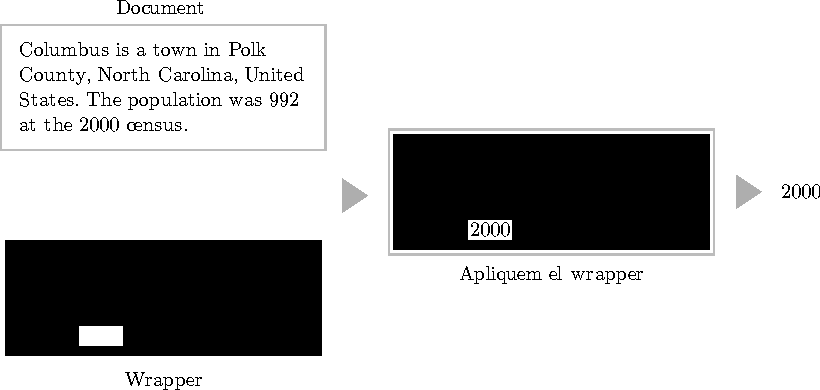
\includegraphics[scale=0.8]{figures/wrapper_sample.pdf}
\caption{Exemple de la funci� d'un \textit{wrapper}}
\label{fig:wrapper-desc}
\end{center}
\end{figure}

A la nostra aplicaci� tindrem els dos tipus de \textit{wrapper} que es descriuen a continuaci�.

\subsection{\textit{Field Wrappers}}
Es tracta de \textit{wrappers} que s'encarreguen d'extreure �nicament un dels camps de la refer�ncia a la vegada. 

En un principi vam comen�ar a implementar aquests \textit{wrappers} manualment, per� aix� comporta diversos problemes:
Aquests 

\subsection{\textit{Reference Wrappers}}
\label{refextraction:reference-wrappers}
Aquest tipus de \textit{wrappers} extreuen el text corresponent a una refer�ncia sencera. El gran avantatge que tenen �s que habitualment permeten extreure molta m�s informaci� i amb una confian�a molt m�s gran.  Ara per ara, el sistema nom�s suporta refer�ncies \BibTeX{}, per� es podria ampliar amb qualsevol altre format.

\paragraph{}
El problema, �s que normalment no es troben a la mateixa p�gina retornada pels cercadors, sin� que cal seguir algun enlla�. A m�s, hi ha moltes biblioteques digitals que no ofereixen les refer�ncies en \BibTeX{} sin� en altres formats com ara \textit{RIS}, \textit{MODS}, etc.



Aquests \textit{wrappers} s'han implementat manualment.



\section{Validaci� de refer�ncies}
\subsubsection{\textit{Parsing} de refer�ncies}
Per poder validar les refer�ncies obtingudes a partir dels \textit{reference wrappers}, �s necessari analitzar-les sint�cticament per tal de poder validar cadascun dels camps. Per aquest motiu, l'aplicaci� disposa d'un \textit{parser} de refer�ncies en format \BibTeX{}.


\section{Format de refer�ncies}

Com a detalls de la implementaci�, nom�s comentar que tindrem un jerarquia de classes anomenades \textit{generadors}; que 
\chapter{Generaci� de \textit{Wrappers}}
\label{chapter:wrapperinduction}

L'usuari sempre podr� corregir els \textit{wrappers} generats per maximitzar la correctesa dels resultats en cada cas.

%%%% OBTENCI� D'EXEMPLES %%%%
\section{Obtenci� d'exemples}
Per poder generar \textit{field wrappers}, es necessiten exemples del camp que es vol extreure. Un exemple est� format pel valor que volem obtenir i pel context en qu� es troba aquest valor. S'obtenen a partir de les refer�ncies emmagatzemades a la base de dades de l'aplicaci�, que poden haver estat importades d'un fitxer \texttt{.bib} o b� extretes anteriorment utilitzant \textit{wrappers} que amb el temps han deixat de funcionar.
Totes les refer�ncies hauran de tenir associada una URL que apunti a una p�gina que cont� la informaci� de la refer�ncia. En el cas de les que s'han obtingut autom�ticament, aquesta adre�a es desa durant l'extracci�.

\paragraph{}
A l'inici, el context dels valors dels nostres exemples �s el document HTML de la p�gina de la refer�ncia. Per tant, el primer pas consisteix en obtenir aquestes p�gines d'Internet. Tot i que per cadascun dels camps es generen \textit{sets} d'exemples diferents, les p�gines s�n les mateixes i nom�s es descarreguen una sola vegada. Tot i aix�, com que totes es trobaran a la mateixa biblioteca i les peticions les procesa el mateix servidor, l'aplicaci� mira d'evitar bloquejos esperant uns segons entre petici� i petici�. Un cop tenim els exemples generats, mirem si el codi HTML cont� la informaci� que volem extreure i si no �s aix�, l'exemple es marca com a inv�lid per tal de no tornar-lo a fer servir en un futur.

\paragraph{}
El codi HTML es neteja per treure'n els comentaris, salts de l�nia, i altres etiquetes que no ens interessen, com ara codi \textit{JavaScript} o etiquetes d'estil. El n�mero d'exemples a tenir en compte per generar els \textit{field wrappers} �s configurable, per� com a m�min es necessiten dos exemples v�lids.

%%%% GENERACI� AUTO. DE REGLES %%%%
\section{Generaci� autom�tica de regles}
Al cap�tol anterior s'ha explicat que els \textit{field wrappers} estan formats per una llista de regles que s'han d'aplicar en un ordre concret per tal de poder extreure el camp que volem. Per nosaltres una regla est� composta per un patr� i un procediment que aplica aquest patr�; en tenim de diferents tipus de regles segons les dades d'entrada i sortida que reben i retornen. Per poder concatenar regles, �s necessari que la sortida d'una regla sigui v�lida per l'entrada de la seg�ent.

\paragraph{}
Els detalls respecte com es creen els regles varien depenent de cada tipus de regla, per� els dos passos b�sics que se segueixen s�n els seg�ents:
\begin{enumerate}
    \item{Genera regles per un dels exemples.}
    \item{Fusiona les �ltimes regles obtingudes amb les anteriors.}
\end{enumerate}
Donat que volem extreure informaci� de documents HTML, les regles que necessitem s�n: una per localitzar l'etiqueta HTML que cont� el valor que ens interessa i una altra per extreure'n aquest valor entre tot el text que pugui acompanyar-lo dins de la mateixa etiqueta. Les hem anomenat \textit{path rules} i \textit{regex rules} respectivament.

\subsection{\textit{Path Rules}}
Aquest tipus de regles s�n les que permeten localitzar trossos d'informaci� dins de la p�gina. Els patrons permeten arribar a l'etiqueta HTML que cont� el valor del camp. Tenen l'aspecte que es mostra a continuaci�, formats per una expressi� regular i una llista de \textit{triplets} compostos pel nom de l'etiqueta, els seus atributs i la posici� respecte els seus \textit{germans}: 
\begin{center}
\begin{lstlisting}
['(\d{4}-\d{3}(\d|X))', (u'table', {u'width': u'100%'}, 7), (u'tr', {}, 0), (u'td', {}, 0)]
\end{lstlisting}
\end{center}

\paragraph{}
Per generar aquests patrons, cerquem el valor que volem extreure dins de l'HTML i anem pujant l'arbre sint�ctic que descriu el document fins arribar a un antecessor amb nom d'etiqueta i atributs �nics. Per cada element en guardem les seves caracter�stiques de manera que despr�s puguem rec�rrer el mateix cam� a l'inrev�s.

\paragraph{}
Pel que fa al n�mero de \textit{sibling} o germ�, nom�s l'utilitzem per agilitzar el proc�s de cerca de la informaci� a l'hora d'aplicar la regla. En un principi hav�em pensat distingir elements segons la seva posici� respecte als germans, per� aix� no funciona en aquells casos on m�ltiples p�gines d'una biblioteca digital mostren la mateixa informaci� en un ordre diferent. Per exemple, si tingu�ssim els dos fragments de codi seg�ents, al cercar el n�mero de volum acabar�em amb les rutes: \texttt{[(table, 0), (tr, \textbf{1}), (td, 0)]} i \texttt{[(table, 0), (tr, \textbf{0}), (td, 0)]}. En realitat, ens interessar� combinar les dues rutes en una de sola i que ens permeti obtenir l'element correcte en qualsevol dels casos. 

\begin{center}
\begin{minipage}{0.48\linewidth}
\begin{lstlisting}[language=HTML, nolol=true]
<table>
  <tr>
    <td class='label'>
      Year:
    </td>
    <td class='value'>
      1985
    </td>
  </tr>
  <tr>
    <td class='label'>
      Volume:
    </td>
    <td class='value'>
      323
    </td>
  </tr>
</table>
\end{lstlisting} 
\end{minipage}
\hspace{0cm}
\begin{minipage}{0.48\linewidth}
\begin{lstlisting}[language=HTML, nolol=true]
<table>
  <tr>
    <td class='label'>
      Volume:
    </td>
    <td class='value'>
      468
    </td>
  </tr>
  <tr>
    <td class='label'>
      Issue:
    </td>
    <td class='value'>
      3
    </td>
  </tr>
</table>
\end{lstlisting}  
\end{minipage}
\end{center}

\paragraph{}
A l'hora de fusionar dos patrons, nom�s ho fem si coincideixen en la llargada, les etiquetes i els atributs dels elements de la ruta. �s a dir, nom�s modifiquem el n�mero de germ�: si dues rutes tenen el mateix n�mero, el deixem tal i com est�; si difereixen, el substitu�m amb el valor $-1$. Si dos patrons no es poden fusionar, acabarem creant \textit{wrappers} diferents amb cadascun d'ells.

\paragraph{}
Mentre apliquem el patr�, si veiem un $-1$ al n�mero de \textit{sibling} fem una cerca de tots els elements d'aquell nivell de l'arbre que compleixen la resta de condicions enlloc d'escollir-ne un directament.  Aix� implica que enlloc d'obtenir un sol element com a resultat, en molts casos en tindrem m�s d'un. Aqu� �s on entra en joc l'expressi� regular de l'inici del patr�. Amb aquesta expressi�, podem ajudar a l'aplicaci� a descartar des d'un principi aquells elements que estem segurs que no ens interessaran. Es pot definir una expressi� regular per cada camp dins del fitxer de configuraci�.

\paragraph{}
Com �s l�gic, en alguns casos ens ser� m�s �til que en altres. Per exemple, si estem intentant extreure l'ISSN d'un article, podem indicar-li l'expressi� \texttt{(\textbackslash{}d\{4\}-\textbackslash{}d\{3\}(\textbackslash{}d|X))}. En canvi, pels valors que no tenen cap tipus d'estructura, com ara els noms de revistes, no ens quedar� cap m�s remei que deixar-ho amb el valor per defecte \texttt{(.*)}

\paragraph{}
Un altre avantatge de tenir aquesta expressi� regular �s que ens servir� per corregir el comportament dels \textit{wrappers} una vegada generats. Per exemple, si veiem que l'any de publicaci� no s'extreu correctament per una biblioteca determinada amb l'expressi� \texttt{(\textbackslash{}d{}4)}, podem restringir m�s el n�mero de coincid�ncies canviant-la per \texttt{(Year\textbackslash{}:\textbackslash{} \textbackslash{}d{4})}


%\begin{center}
%\begin{lstlisting}[caption={\textit{Merging} de \textit{path rules}}]
%Els patrons
%['(.*)', (u'table', {}, 7), (u'tr', {}, 2), (u'td', {}, 0)]
%['(.*)', (u'table', {}, 7), (u'tr', {}, 3), (u'td', {}, 0)]
%
%Quedaria:
%[['(.*)', (u'table', {}, 7), (u'tr', {}, -1), (u'td', {}, 0)]]
%
%En canvi:
%['(.*)', (u'table', {}, 7), (u'tbody', {}, 0), (u'tr', {}, 2), (u'td', {}, 0)]
%['(.*)', (u'table', {}, 7), (u'tr', {}, 3), (u'td', {}, 0)]
%
%Quedaria:
%[['(.*)', (u'table', {}, 7), (u'tbody', {}, 0), (u'tr', {}, 2), (u'td', {}, 0)],
% ['(.*)', (u'table', {}, 7), (u'tr', {}, 3), (u'td', {}, 0)]]
%
%\end{lstlisting}
%\end{center}



\subsection{\textit{Regex Rules}}
Aquestes regles permeten extreure un camp quan el valor d'aquest es troba dins d'un element del document HTML acompanyat de m�s text. Reben una o m�s cadenes de car�cters com a entrada i els hi apliquen una expressi� regular generada autom�ticament per tal de quedar-se nom�s amb una part la cadena.  

\paragraph{}
Per generar les expressions regulars, s'agafa el text contingut als elements HTML que ens proporcionen les \textit{path rules} i es fa una substituci� del valor que volem obtenir per l'expressi� \texttt{(.*)}. Per exemple, si volgu�ssim obtenir el n�mero de p�gines d'una p�gina que cont� la l�nia seg�ent, comen�ar�em posant els car�cters d'escapament necessaris i substituint el valor \texttt{1204-1209}.

\begin{center}
\begin{lstlisting}[nolol=true]
Vol. 27, No. 6. (1 April 2006), pp. 1204-1209.

Vol\.\ 27\,\ No\.\ 6\.\ \(1 April 2006\)\,\ pp\. (.*)\.
\end{lstlisting}
\end{center}
De moment, com que nom�s hem generat l'expressi� amb una sola regla, no �s prou general per extreure els camps de totes les p�gines. A a mesura que es provi amb m�s exemples, els trossos de text que varien aniran desapareixent. Suposem que ens arriba un altre exemple i la \textit{path rule} ens retorna la l�nia seg�ent, per la qual tamb� en generem l'expressi�.

\begin{center}
\begin{lstlisting}[nolol=true]
Vol. 24, No. 1. (2 March 1999), pp. 332-344.

Vol\.\ 31\,\ No\.\ 1\.\ \(2 March 1999\)\,\ pp\. (.*)\.
\end{lstlisting}
\end{center}

A simple vista veiem que es tracta a la mateixa part de la p�gina HTML que la de l'exemple anterior, i que haur�em de poder aplicar la mateixa expressi� regular en els dos casos per tal d'obtenir el n�mero de p�gines. La t�cnica que fem servir per decidir si hem de fusionar dues expressions �s molt simplista, tan sols avaluem la similaritat de les expressions i comprovem si supera un llindar establert. De ser aix�, obtenim els blocs no coincidents de les dues cadenes de car�cters i els substitu�m per \texttt{(?:.*)} que amb \textit{Python} indica que es pot acceptar qualsevol cadena, per� que cal descartar-la a l'hora de retornar els grups coincidents. El resultat de fusionar les dues expressions �s:

\begin{center}
\begin{lstlisting}[nolol=true]
Vol\.\ (?:.*)\,\ No\.\ (?:.*)\.\ \((?:.*)r(?:.*)\)\,\ pp\. (.*)\.
\end{lstlisting}
\end{center}

Com es pot veure, encara ha quedat la lletra \textit{r} entre dos blocs a descartar. Durant la fusi� d'expressions el sistema tamb� aplica heur�stiques que ajuden a generalitzar m�s r�pid. Per exemple, quan troba blocs coincidents de llargada 1, formats per una lletra o un n�mero, els elimina. Per altra banda, tamb� s'agrupen els blocs consecutius a descartar. L'expressi� final resultant queda:
\begin{center}
\begin{lstlisting}[nolol=true]
Vol\.\ (?:.*)\,\ No\.\ (?:.*)\.\ \((?:.*)\)\,\ pp\. (.*)\.
\end{lstlisting}
\end{center}

\paragraph{}
Aquest m�tode de generar les expressions regulars no est� exempt de problemes i es podria millorar per convergir a una expressi� m�s general i fent servir menys exemples. En un principi gener�vem les expressions de forma creixent, agafant el valor a extreure, i mirant els primers car�cters de la vora (aquesta �s una simplificaci� de com ho feia el sistema \textit{WHISK}\cite{soderland99}). El problema el ten�em quan la informaci� del context tamb� variava entre p�gina i p�gina. Per tant, tot i ser una forma m�s r�pida de crear les regles, no ens donava resultats prou bons. A la llarga es podria mirar d'utilitzar una aproximaci� intermitja, agafant el context m�nim de l'expressi� generada amb el m�tode actual. D'aquesta manera reduir�em el n�mero d'exemples necessaris per arribar a expressions regulars prou generals.
\begin{center}
\begin{lstlisting}[nolol=true]
\ pp\. (.*)\.
\end{lstlisting}
\end{center}

No obstant, hem de comentar que l'aplicaci� permet l'edici� de regles per part de l'usuari. De manera que si una expressi� regular no s'ha acabat de generar prou b�, sempre es pot modificar.

\subsection{Regles multi valor}
Alguns camps com ara els autors o editors tenen m�ltiples valors. Per poder-los extreure per separat, hem creat variants de les regles anteriors.  Assumim que els m�ltiples valors corresponents al mateix cam copmliran una de les dues condicions seg�ents:
\begin{itemize}
\item{}
Es troben en elements HTML diferents, per� s�n germans o cosins. Aquesta condici� permet extreure valors quan es troben tant en llistes com en taules:
\begin{center}
\begin{minipage}{0.45\linewidth}
\begin{lstlisting}[language=HTML, title={Germans}, nolol=true]
<ul>
  <li>
    Liu Jing
  </li>
  <li>
  Li Jiandong
  </li>
  <li>
    Chen Yanhui
  </li>
</ul>
\end{lstlisting} 
\end{minipage}
\begin{minipage}{0.53\linewidth}
\begin{lstlisting}[language=HTML, title={Cosins}, nolol=true]
<table>
  <tr>
    <td>Autors:</td>
    <td>Liu Jing</td>
  </tr>
  
  <tr>
    <td></td>
    <td>Li Jiandong</td>
  </tr>
</table>
\end{lstlisting}  
\end{minipage}
\end{center}

\item{}
Es troben dins el mateix HTML amb un o m�s separadors entre ells. Per exemple, els tres autors seg�ents estan separats per les cadenes ``, '' i `` and ''.
\begin{center}
\begin{lstlisting}[language=HTML, caption={Exemple m�ltiples valors}, label=listing:exampleSiblingElements]
<td>Liu Jing, Li Jiandong and Chen Yanhui</td>
\end{lstlisting}
\end{center}

\end{itemize}

\paragraph{}
La t�cnica per generar les regles per obtenir els elements HTML �s molt semblant a les que ja hem explicat pels camps d'un sol valor. L'�nica difer�ncia �s que cal realitzar \textit{merging} dels patrons dels m�ltiples valors dins de la mateixa p�gina.

\paragraph{}
Pel que fa a les \textit{regex rules}, les substitu�m per:
\begin{itemize}
\item{\textit{Separator rules}:} S�n les encarregades de dividir l'entrada en m�ltiples valors segons una s�rie de separadors. El seu patr� consisteix en una llista amb aquests separadors.

\item{\textit{Multi-value regex rules}:} Acompleixen la mateixa funci� que les \textit{regex rules} de l'apartat anterior, per� amb la difer�ncia que reben i retornen m�ltiples valors. L'expressi� regular del patr� s'aplica per cadascun dels valors.

\item{\textit{Person rules}:} Nom�s s'apliquen en el cas dels autors i els editors. Reben el nom complet d'una persona i s'encarreguen de separar-lo les diferents part del nom. Es consideren les parts: \textit{first name}, \textit{middle name} i \textit{last name}. Tenir els noms separats permet que a l'hora de generar la refer�ncia \BibTeX{} tots els noms estiguin en el mateix format. A continuaci� es mostren exemples de com quedarien dos noms:
\begin{center}
\begin{minipage}{0.45\linewidth}
\begin{lstlisting}[nolol=true]
David P. Bartel

{u'first_name':
   u'David',
 u'middle_name':
   u'P.',
 u'last_name':
   u'Bartel'}
\end{lstlisting}
\end{minipage}
\hspace{0cm}
\begin{minipage}{0.45\linewidth}
\begin{lstlisting}[nolol=true]
James Green

{u'first_name':
   u'James',
 u'middle_name':
   u'',
 u'last_name':
   u'Green'}
\end{lstlisting}
\end{minipage}
\end{center}

\end{itemize}

\section{Avaluaci� dels \textit{wrappers}}
Una vegada hem generat el conjunt dels \textit{wrappers} possibles per a cadascun dels camps, cal que avaluem quins d'ells funcionen millor. Primer, els avaluem amb els mateixos exemples que hem fet servir per la generaci�. Aix� ens donar� una idea o confian�a sobre com poden arribar a funcionar a l'hora de la veritat i ens guiar� a l'hora d'escollir quins aplicar primer. Durant l'extracci� de refer�ncies, cada vegada que s'utilitza un \textit{wrapper} s'avalua la informaci� que ha extret i es corregeix la valoraci� sobre el funcionament d'aquest \textit{wrapper}.

\paragraph{}
El sistema d'avaluaci� �s molt senzill, per cadascuna de les vegades que s'extreu informaci� amb �xit es d�na un vot positiu. Si la informaci� no �s correcta, se li'n d�na un de negatiu. La puntuaci� del \textit{wrapper} ser� el percentatge de vots positius.
\begin{equation*}
    score = \frac{vots\; positius}{vots\; totals}
\end{equation*}

\paragraph{}
Amb aquesta manera de calcular la puntuaci�, hem de ser conscients del quue passa quan comparem \textit{wrappers} molt utilitzats amb altres que no ho han estat tant. Per exemple, si tenim un \textit{wrapper} que ha funcionat moltes vegades durant el passat (molts vots positius) i comen�a a fallar, el percentatge decreixer� i de seguida es donar� pas a un altre \textit{wrapper} menys usat, per� que no t� vots negatius. Per resoldre aix�, nombrosos llocs web usen el \textit{Wilson score interval} descrit a \cite{miller09} per ordenar elements.

\paragraph{}
Si ens parem a pensar, per�, aquest comportament �s probablement el que realment busquem. Quan un \textit{wrapper} comen�a a fallar, �s molt probable que ho faci degut a algun canvi en l'estructura de les p�gines de les quals extreu la informaci�. Si �s aix�, ja sabem que aquest \textit{wrapper} no tornar� a funcionar m�s i ens interessa descartar-lo tant r�pid com sigui possible. Tamb� podem agilitzar-ho donant m�s vots negatius que negatius.


\chapter{An�lisi de resultats}
\label{chapter:results}
%En aquest cap�tol es mostren les principals proves realitzades per cadascuna de les tres parts del sistema descrites als cap�tols anteriors. Aqu� s'intenten mostrar nom�s una mostra dels rsultats obtinguts i alguns casos interessants. La resta es troba a l'ap�ndix \ref{appendix-results}.


%%%% REFERENCE SEARCH %%%%
\section{Cerca de refer�ncies}
\label{chapter:results:section:search}
En primer lloc provarem com de b� ho fa el sistema a l'hora de cercar p�gines a Internet que continguin informaci� sobre un article concret. Els tests que hem dut a terme consisteixen en els passos seg�ents:
\begin{enumerate}
\item{Obtenir una s�rie de consultes per cadascun dels articles d'un llistat de PDFs}
\item{Cercar cada consulta amb els tres cercadors implementats: \textit{Google}, \textit{Bing} i \textit{Yahoo}}
\item{Per cada resultat obtingut, analitzem si �s bo o no}
\item{Comptabilitzem el n�mero de consultes que han fet falta per obtenir el primer \textit{bon} resultat}
\end{enumerate}

Per tal de classificar els resultats en bons i dolents nom�s comprovem si algunes porcions de la informaci� que volem es troben dins de la p�gina resultant. Aquesta no �s una soluci� perfecta, per� ens permet fer una aproximaci� sobre la quantitat de fitxers pels quals podem trobar la refer�ncia.

\paragraph{}
Una altra q�esti� sobre la implementaci� d'aquestes proves, �s que els resultats obtinguts se solen repetir entre consultes del mateix article. Per estalviar temps i evitar fer moltes peticions seguides als mateixos servidors (que podrien resultar en un bloqueig), deixem uns quants segons entre petici� i petici� i emmagatzemem cada resultat de manera que nom�s l'h�gim de demanar una sola vegada. A banda d'aix�, tamb� cal tenir en compte que en molts casos els resultats corresponen al mateix fitxer PDF del qual estem buscant informaci�, els hem d'ometre.

\paragraph{}
Aquests tests s'han realitzat per conjunts d'articles diferents agrupats depenent de la seva cap�alera, que �s el que pot fer variar m�s els resultats obtinguts. Hi ha un �ltim grup que cont� articles de qualsevol tipus. Aqu� nom�s es mostren les dades d'aquest darrer conjunt a les figures \ref{fig:results:random-reslen} i \ref{fig:results:random-fqlen}, per� a l'ap�ndix de resultats (\ref{appendix-results}) tamb� hi ha els gr�fics per dos m�s d'aquests conjunts.

\begin{figure}[H]
\begin{center}
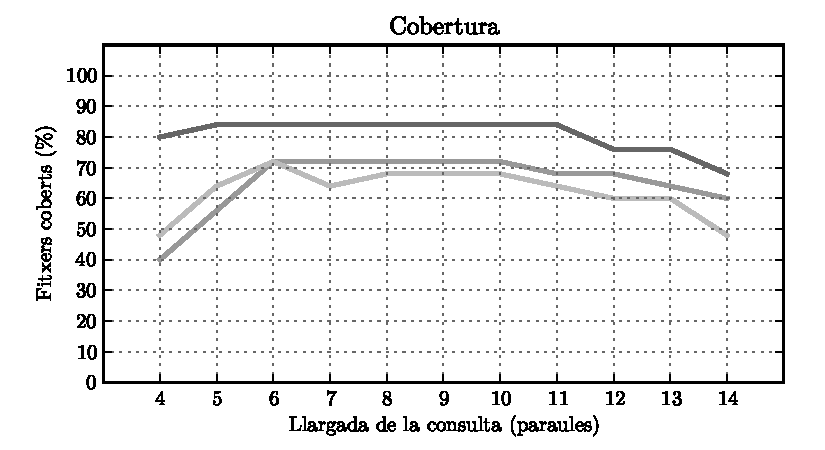
\includegraphics[width=0.8\textwidth]{figures/results:random-reslen.pdf}
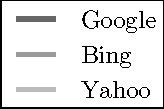
\includegraphics[scale=0.8]{figures/results:search-legend.pdf}
\caption{Comparaci� de la qualitat dels resultats obtinguts segons la llargada de les consultes}
\label{fig:results:random-reslen}
\end{center}
\end{figure}

El primer gr�fic mostra el percentatge de fitxers del conjunt provat pels quals s'ha obtingut almenys un bon resultat. Tot i que aqu� no es vegi, en algunes ocasions els resultats bons retornats per \textit{Bing} o \textit{Yahoo} han estat superiors en nombre, el que s� que veiem, per�, �s que en general, el cercador \textit{Google} ofereix major cobertura amb resultats sobre m�s articles diferents.

\begin{figure}[H]
\begin{center}
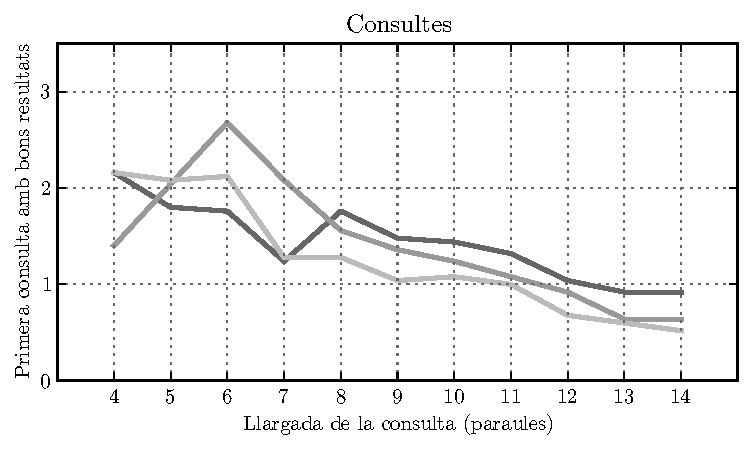
\includegraphics[width=0.8\textwidth]{figures/results:random-fqlen.pdf}
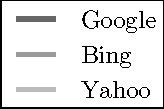
\includegraphics[scale=0.8]{figures/results:search-legend.pdf}
\caption{Comparaci� del n�mero de consultes necess�ries abans de trobar bons resultats}
\label{fig:results:random-fqlen}
\end{center}
\end{figure}

En el segon gr�fic veiem que pel que fa a les consultes, el n�mero de cerques que hem de fer per comen�ar a obtenir bons resultats minva a mesura que es fan servir m�s paraules. De totes maneres, tal i com ja s'ha dit a la secci� \ref{chapter:search:skip-queries}, �s bo que ens saltem les primeres consultes per evitar cercar amb el t�tol de l'article i anar directament al resum o \textit{abstract}.



%%%% WRAPPER INDUCTION %%%%
\section{Generaci� de \textit{wrappers}}
\label{chapter:results:section:wrapperinduction}
Per provar aquesta part del sistema, hem creat conjunts de p�gines web amb informaci� d'articles diferents i amb la refer�ncia corresponent. Cada grup inclou nom�s p�gines corresponents a la mateixa biblioteca digital i per cadascun d'ells n'hem importat les refer�ncies i hem generat els \textit{wrappers} pels diferents camps. 

\paragraph{}
Les mostres no s�n gaire significatives, per� ens donen una idea per poder quantificar com de b� funciona la nostra eina dins l'entorn pel qual est� pensat. Les proves d'aquesta secci� corresponen a les puntuacions rebudes durant l'avaluaci� dels \textit{wrappers} i permeten marcar un ordre d'elecci� inicial a l'hora d'extreure refer�ncies. Com que de moment encara no hem fet proves amb p�gines que no s'han emprat per la generaci� (ho farem a la propera secci�), els gr�fics no indiquen la correctesa dels resultats dels \textit{wrappers} sin� la \textit{confian�a} que tenim en que funcionin. Recordem que els camps obligatoris que han de contenir les refer�ncies a articles s�n: \textit{author}, \textit{title}, \textit{journal} i \textit{year}; per aquest motiu, aquests s�n els camps en que ens centrarem.

\begin{figure}[H]
\begin{center}
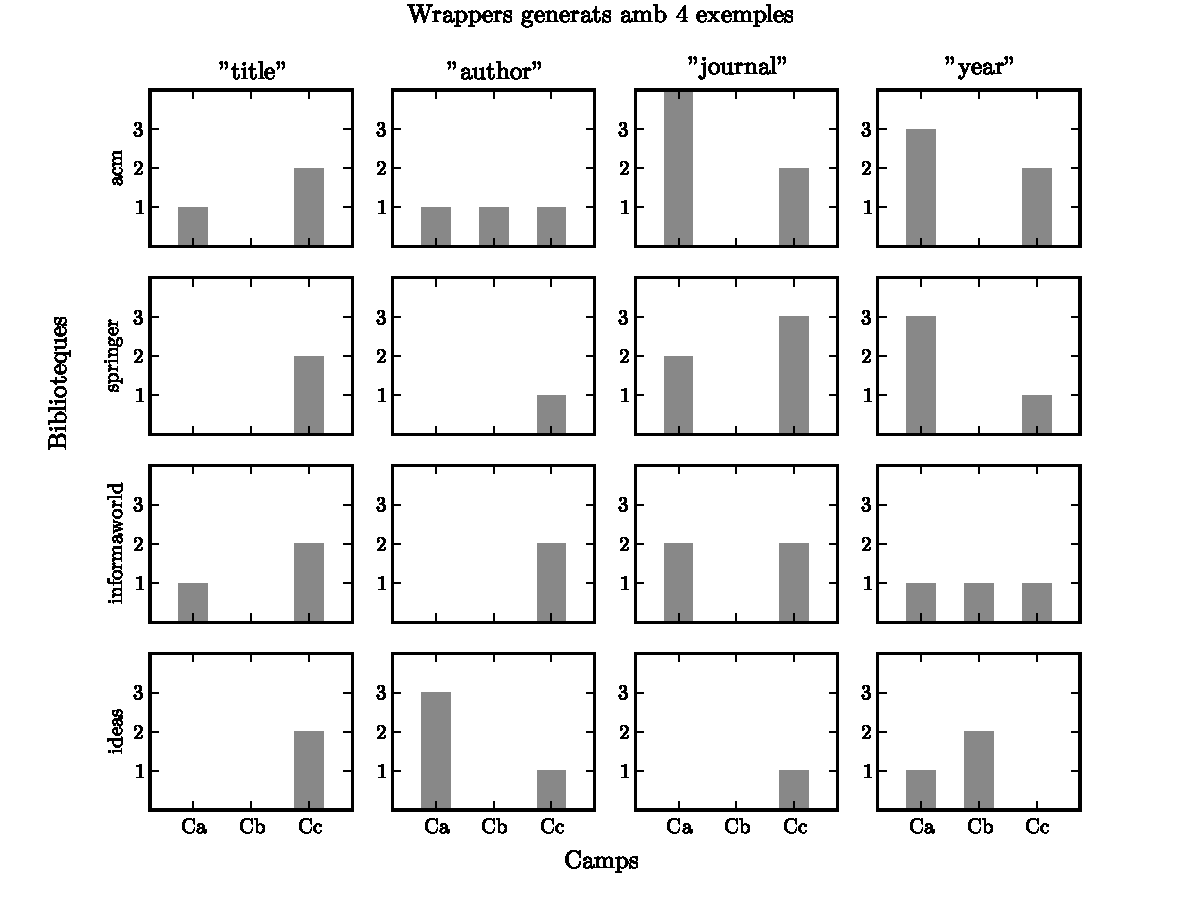
\includegraphics[width=0.8\textwidth]{figures/results:nwrappers-4.pdf}
%\caption{Nombre de \textit{Wrappers} generats utilitzant 4 exemples i agrupats per confian�a}
\label{fig:results:nwrappers-4}
\end{center}
\end{figure}

El primer gr�fic permet comparar el n�mero de \textit{wrappers} obtinguts per cadascun dels camps per diferents biblioteques i utilitzant 4 exemples al generar. Tal i com es pot veure a la llegenda, els hem classificat en diferents grups de confian�a, depenent de la puntuaci� rebuda a l'avaluar-los amb els mateixos 4 exemples. S'han om�s aquells que no han funcionat en cap cas. Aqu� ens interessa veure, sobretot, si hi ha almenys un \textit{wrapper} de confian�a \textit{Cc}. Quan n'hi ha m�s d'un, solen indicar que les dades estan repetides dins la p�gina i que, per tant, hi ha diverses formes de poder-les extreure. En el cas del camp \textit{title} de la biblioteca \textit{acm}, el t�tol es troba a l'etiqueta \texttt{<title>} i dins d'alguna altra etiqueta dins el \texttt{<body>} de la p�gina.

\paragraph{}
El gr�fic tamb� mostra dos casos pels quals no s'ha obtingut cap \textit{wrapper} que hagi funcionat per tots els exemples: el camp \textit{author} de la biblioteca \textit{InformaWorld} i el camp \textit{year} d'\textit{Ideas}. Amb una ullada r�pida a les regles generades n'hi ha prou per veure que es tracta de problemes de generalitzaci�. Pel cas del camp corresponent a l'any, les expressions regulars de les dues \textit{regex rules} s�n:

\begin{center}
\begin{lstlisting}[nolol=true]
"Handle\:\ RePEc\:tov\:dsiess\:v\:3\:y\:(.*)"
\end{lstlisting}
\begin{lstlisting}[nolol=True]
"Handle\:\ RePEc\:(?:.*)af\:(?:.*)v\:(?:.*)\:y\:(.*)"
\end{lstlisting}
\end{center}

Aquest �s el problema que s'ha descrit a la secci� \ref{chapter:wrapperinduction:section:regexrules} al parlar de la generaci� d'expressions regulars. Els patrons inicials eren massa diferents com per fusionar-los i s'ha acabat amb regles massa espec�fiques. Si ho correg�ssim manualment, l'expressi� resultant seria:
\begin{center}
\begin{lstlisting}[nolol=true]
"Handle\:\ RePEc\:(?:.*)\:y\:(.*)"
\end{lstlisting}
\end{center}

Aqu� queda plasmada ara la import�ncia d'escollir bons exemples per la generaci� de regles. A l'ap�ndix \ref{fig:results:nwrappers-2} hi ha la mateixa gr�fica, per� pertanyent als \textit{wrappers} obtinguts utilitzant nom�s $2$ exemples. Els resultats s�n similars.  

\begin{figure}[H]
\begin{center}
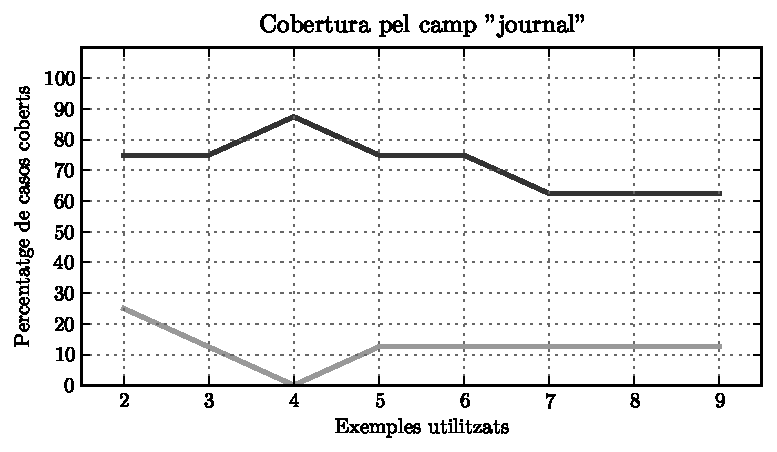
\includegraphics[width=0.8\textwidth]{figures/results:coverage-journal.pdf}
\caption{Cobertura dels \textit{wrappers} pel camp \textit{journal}}
\label{fig:results:coverage-journal}
\end{center}
\end{figure}

\paragraph{}
A part d'aquesta vista dels resultats m�s detallada, les gr�fiques \ref{fig:results:coverage-journal} i \ref{fig:results:coverage-year} tamb� mostren el percentatge de biblioteques provades per les quals s'han obtingut \textit{wrappers} de confian�a, depenent del n�mero d'exemples utilitzats per la generaci�. La l�nia fosca indica el percentatge de les biblioteques digitals per les quals hem obtingut almenys un \textit{wrapper} de confian�a m�xima, la l�nia m�s clara indica el mateix percentatge, per� del seg�ent interval de confian�a. Finalment, la l�nia discontinua representa la suma de les dues anteriors.

\paragraph{}
El camp corresponent a l'any �s interessant perqu� moltes de les p�gines que hem provat contenen m�ltiples aparicions del valor que busquem, per� no sempre descrivint l'any de publicaci�, sin� la data de revisi�, la data a partir de la qual l'article es troba a Internet, \textit{copyright}, etc.
Aquest tipus de confusions tamb� s�n habituals quan, a m�s de la informaci� de l'article, les p�gines inclouen llistats amb les citacions o refer�ncies a d'altres publicacions. Malgrat tot, a mesura que comencem a tenir m�s exemples el fet d'avaluar ens permetr� escollir aquells valors que realment s�n v�lids.

\paragraph{}
Altres camps pels quals es t� m�s dificultat per generar \textit{wrappers} s�n aquells el valor dels quals consisteix en n�meros petits, com ara el n�mero de volum (\texttt{volume}) o de revista (\texttt{number}). El motiu �s el mateix, hi ha moltes aparicions del valor, per� que no fan refer�ncia al camp que busquem.


\begin{figure}[H]
\begin{center}
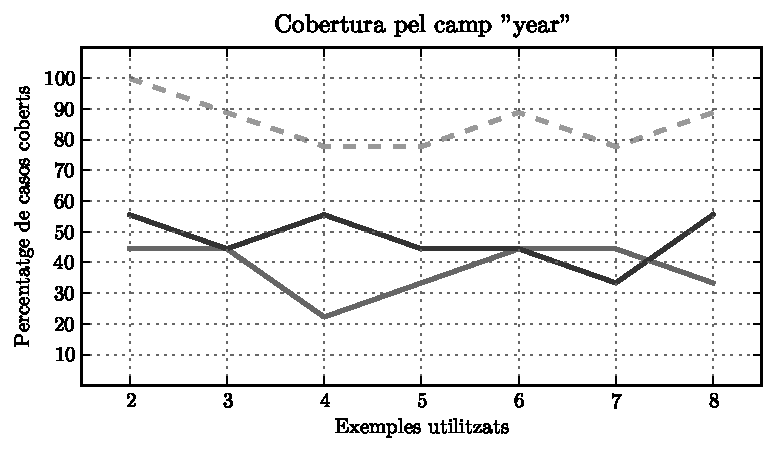
\includegraphics[width=0.8\textwidth]{figures/results:coverage-year.pdf}
\caption{Cobertura dels \textit{wrappers} pel camp \textit{year}}
\label{fig:results:coverage-year}
\end{center}
\end{figure}


%%%% REFERENCE EXTRACTION %%%%
\section{Extracci� de refer�ncies}
Anem a veure ara com de b� ho fan els \textit{wrappers} generats a la secci� anterior a l'hora d'extreure informaci� per les mateixes biblioteques i camps. Disposem de conjunts de p�gines d'articles diferents i les seves refer�ncies en \BibTeX{}, que faran de mostres de control per saber en quins casos s'ha encertat i en quins no. Com que en aquest punt els resultats s�n m�s interessants, hem incl�s els gr�fics de 2 i 4 exemples aqu� mateix. Per comen�ar ens fixarem en la correctesa dels camps extrets amb regles generades a partir de dos exemples:

\begin{figure}[H]
\begin{center}
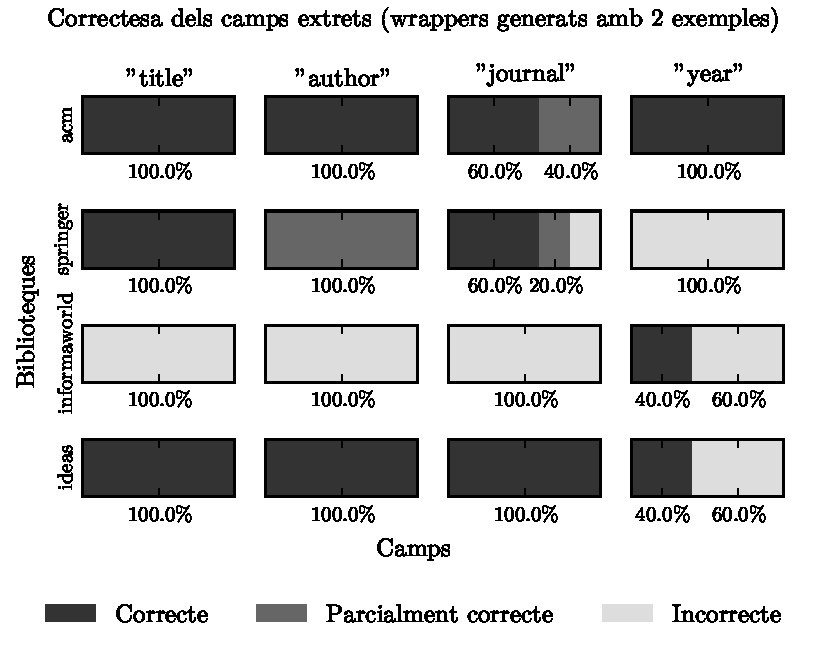
\includegraphics[width=0.8\textwidth]{figures/results:extraction-2.pdf}
%\caption{Camps extrets amb els \textit{wrappers} generats amb 2 exemples}
\label{fig:results:extraction-2}
\end{center}
\end{figure}

Es considera que el valor extret �s:
\begin{itemize}
\item{\textit{Correcte}:}
Quan el valor obtingut coincideix exactament amb el de la refer�ncia de control.
\item{\textit{Parcialment correcte}:}
Si el text extret cont� el valor de control a m�s d'altra informaci�. Per exemple, un dels valors extrets pel camp \textit{journal} de la biblioteca \textit{ACM} �s: \texttt{ACM Computing Surveys \textbf{(CSUR)}} mentre que el valor de la refer�ncia de control �s \texttt{ACM Computing Surveys}. Tot i que en situacions com aquestes els valors es podrien considerar correctes, s'ha decidit generar els gr�fics aplicant les regles de classificaci� de forma estricta i comentar-ho si fa falta.
\item{\textit{Incorrecte}:}
en qualsevol altre cas.
\end{itemize}


Veiem que utilitzant dos exemples hi ha hagut for�a problemes, tots per culpa que les regles s�n massa espec�fiques com per cobrir nous casos:
\begin{itemize}
\item{}
Com ja s'ha anticipat a la secci� anterior, un dels camps amb m�s problemes ha estat l'any, que no s'ha pogut extreure correctament en tres de les quatre biblioteques que es mostren per culpa que no s'ha escollit b� l'element HTML que realment cont� aquesta informaci�.
\item{}
 Els autors de la biblioteca \textit{SpringlerLink} no s'han extret del tot b� en cap dels casos, per culpa que els separadors de les \textit{separator rules} no s�n prou gen�rics.
\item{}
Per acabar, els resultats de la biblioteca \textit{InformaWorld} s�n p�ssims a causa de combinacions dels dos problemes anteriors.
\end{itemize} 

Anem a veure qu� passa quan fem les mateixes proves amb els \textit{wrappers} generats a partir de quatre exemples diferents:

\begin{figure}[H]
\begin{center}
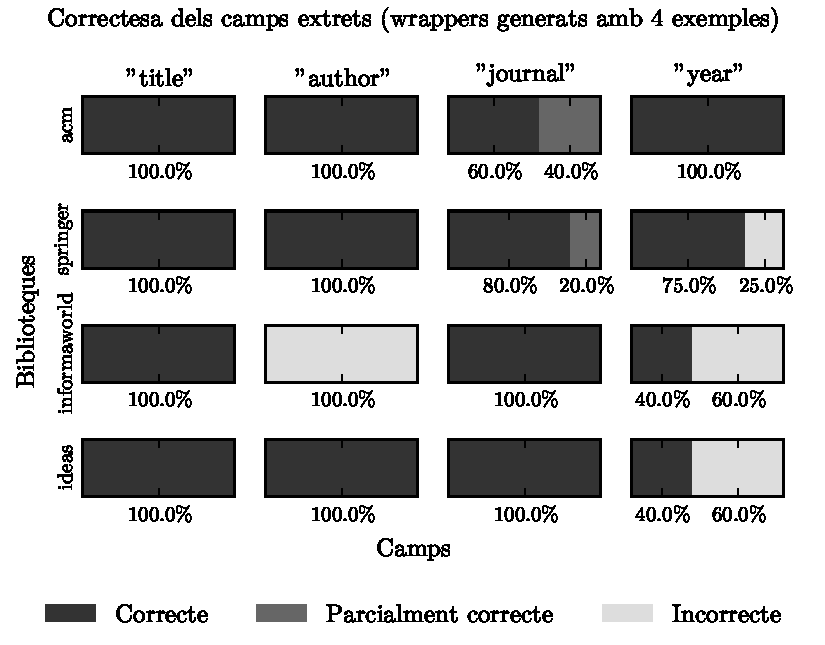
\includegraphics[width=0.8\textwidth]{figures/results:extraction-4.pdf}
\label{fig:results:extraction-4}
\end{center}
\end{figure}

El nombre d'extraccions correctes ha augmentat for�a, i els valors marcats com a \textit{parcialment correctes} corresponen a situacions que realment es podrien considerar v�lides. En canvi, segueixen havent-hi problemes amb els anys i amb els autors de la biblioteca \textit{InformaWorld}. Podem mirar de corregir-los manualment.

\paragraph{}
Respecte als autors d'\textit{InformaWorld} no s'ha sabut identificar correctament l'element HTML que els cont�. Nom�s canviant l'expressi� regular de l'inici de la \textit{path rule}, per ajudar a escollir l'element adequat, passem a extreure els autors de forma correcta per a tots els casos.
\begin{center}
\begin{lstlisting}[nolol=true]
[".*", ["div", {"id": "metahead"}, 0], ...
\end{lstlisting}
\begin{lstlisting}[nolol=true]
["Authors?:\ (.*)", ["div", {"id": "metahead"}, 0], ...
\end{lstlisting}
\end{center}


\paragraph{}
En relaci� amb l'any de publicaci�, el problema consisteix, una vegada m�s, en una expressi� regular massa espec�fica. La canviem per una de m�s general:
\begin{center}
\begin{lstlisting}[nolol=true]
"Published\ in\:Accounting\ Education\,\ Volume\ \ 1(?:.*)\,\ Issue\ \ (?:.*)\ \&\ (?:.*)\ \ (?:.*)\ (.*)\ \,\ pages\ (?:.*)\ \-\ "
\end{lstlisting}
\begin{lstlisting}[nolol=true]
"\ (\d{4})\ \,\ pages\ "
\end{lstlisting}
\end{center}

Un cop fetes aquestes correccions, si tornem a executar les proves per extreure les refer�ncies, obtenim un 100\% d'encerts pels quatre camps que hem tractat.
\begin{figure}[H]
\begin{center}
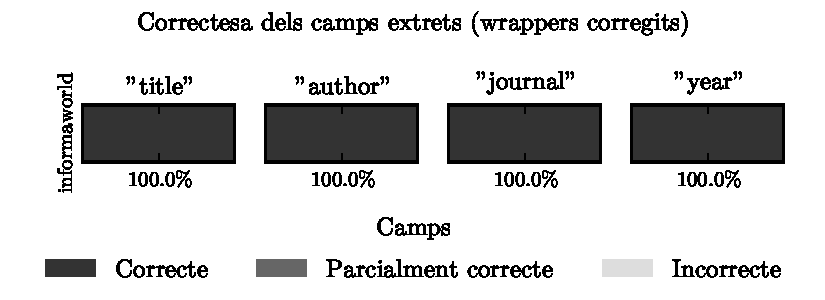
\includegraphics[width=0.8\textwidth]{figures/results:extraction-corrected.pdf}
%\caption{Camps extrets per la biblioteca \textit{InformaWorld} despr�s de corregir els \textit{wrappers}}
\label{fig:results:extraction-corrected}
\end{center}
\end{figure}

Els resultats d'extracci� dels camps que no es mostren als gr�fics (e.g. n�mero de volum, p�gines) s�n molt similars als que acabem de veure. El n�mero de revista i volum tenen problemes similars als del camp referent a l'any, en canvi, altres menys comuns com ara l'ISSN tenen una taxa d'encerts molt alta.


%%% GENERAL %%%%
\section{Funcionament de tot el sistema}
\label{appendix:results:section:wholesystem}
Acabem de veure com ho fa la nostra aplicaci� per cadascun dels problemes a solucionar per aconseguir l'objectiu d'extreure refer�ncies. Aqu� es mostren els resultats obtinguts una vegada hem unit les tres parts anteriors. Per realitzar les proves s'ha creat un conjunt aleatori de fitxers PDF corresponents a articles relacionats amb el camp de la inform�tica. Aix� afecta bastant a les biblioteques per les quals es trobaran resultats, ja que molts articles d'aquest tipus acostumen a estar indexats per \textit{ACM Portal}, \textit{SpringerLink} i \textit{CiteSeerX}.

\paragraph{}
Els tres gr�fics seg�ents exposen els resultat depenent de l'estat de l'aplicaci�: el primer, quan no hi ha cap \textit{fiel wrapper} definit; el segon, una vegada hem generat \textit{field wrappers} per les p�gines que m�s s'utilitzen; i la tercera, un cop hem corregit algunes de les regles manualment.


\begin{figure}[H]
\begin{center}
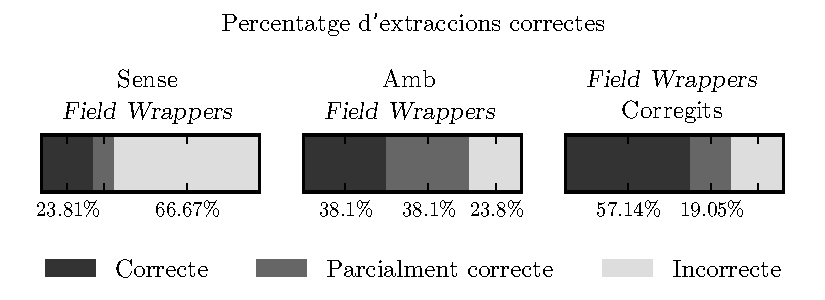
\includegraphics[width=0.8\textwidth]{figures/results:general-extraction.pdf}
%\caption{Camps extrets per la biblioteca \textit{InformaWorld} despr�s de corregir els \textit{wrappers}}
\label{fig:results:general-extraction}
\end{center}
\end{figure}

Es considera que una refer�ncia s'ha extret de forma correcta si tots els quatre obligatoris tenen el valor esperat. Parcialment correcta, si algun d'aquests camps no hi �s present, o b� t� un valor incorrecte, per� la resta estan b�. I incorrecta, altrament.

\paragraph{}
El temps necessari per executar pot variar segons la connexi� a Internet de la qual es disposa, tot i que en situacions \textit{normals} el temps mitj� per fitxer sol estar entre 1 i 1.5 segons. Una de les conseq��ncies de fer servir diferents fils d'execuci� �s que si l'espera d'algun dels fitxers tarda m�s del compte, els altres es poden anar processant.


\chapter{Conclusions i treball futur}
\label{chapter:conclusions}

Al llarg d'aquest document s'han descrit les decisions que hem pres i el proc�s seguit per poder implementar una aplicaci� d'extracci� de refer�ncies. Part�em d'aquest objectiu �nic i, per tant, tot el que hem anat fent gira al voltant d'aquesta idea: l'extracci� de text dels PDFs, la cerca d'articles en biblioteques digitals i tamb� l'extracci� d'informaci� dins de documents HTML.

\paragraph{}
En part, podr�em dir que el proc�s d'extracci� s'ha basat en un c�mul d'assumpcions que, dins del context de l'aplicaci�, es compleixen en la gran majoria de casos. De totes maneres, cal tenir en compte que el procediment que se segueix es veu afectat, a cada pas, per p�rdues inevitables:
\begin{itemize}
\item{}
L'extracci� del text dels fitxers PDF no es pot fer per documents formats per imatges que han estat escanejats sense utilitzar \textit{software} de reconeixement de car�cters.
\item{}
El pas de cercar el document a Internet requereix, com �s l�gic, que es trobi en alguna de les biblioteques digitals indexades pels cercadors. Es descartar� qualsevol escrit pel qual no es trobin resultats.
\item{}
Per �ltim, pel que fa a extreure informaci� de les p�gines HTML de forma correcta, ja hem vist que dep�n molt de les regles que tinguem definides, per� que els resultats tampoc no s�n perfectes.
\end{itemize}
Al final, hem aconseguit una eina que funciona i que, tal i com hem pogut comprovar, obt� resultats mitjanament bons. L'�xit de regles generades per a l'extracci� varia segons el tipus de dades a obtenir. Mentre els camps com ara el t�tol, autors, nom de revista, etc. tenen una taxa d'encerts for�a elevada, altres camps com l'any de publicaci�, n�mero de volum o n�mero de la revista porta m�s problemes.

\paragraph{}
Cal comentar que, tot i que el sistema est� destinat a l'extracci� de refer�ncies, la part de generaci� de regles i la manera d'aplicar-les podria ser, en realitat, la base d'un \textit{framework} �til per qualsevol altra eina similar d'extracci� d'informaci� estructurada. En cas de no tractar-se de documents HTML, nom�s caldria afegir els nous tipus de regles necessaris.

\paragraph{}
Un altre punt interessant �s que, al tractar-se d'un projecte \textit{open source}, qualsevol persona interessada es pot dirigir al repositori p�blic que hi ha a \textit{GitHub} (\cite{repo}) i fer un \textit{fork} per desenvolupar noves funcionalitats o b� arreglar errors. Si es tracta d'un treball derivat haur� de distribuir-se sota les mateixes condicions.

\section{Possibles Millores}
Des d'un punt de vista objectiu, el sistema encara hauria de passar per m�s iteracions abans de poder-lo considerar s�lid. Alguns dels aspectes que s'haurien de tractar primer s�n:

\begin{itemize}
\item{}
El primer i m�s important seria incorporar millores a la generaci� d'expressions regulars a partir d'exemples per tal d'aconseguir expressions generals utilitzant pocs exemples.
\item{}
Possibilitat d'actualitzar \textit{wrappers} a mesura que es disposa de nous exemples. Quan una refer�ncia s'extreu correctament de forma autom�tica significa que les regles funcionen, per� quan hi ha errors i l'usuari fa correccions, l'aplicaci� hauria de ser capa� d'adonar-se'n i actualitzar-se per fer-ho b� en pr�ximes execucions. Hauria de ser capa� d'aprendre.
\item{}
Suportar altres llenguatges de citacions no nom�s suposaria poder importar i exportar refer�ncies amb aquests formats sin� que permetria que els \textit{reference wrappers} que hem descrit a la secci� \ref{refextraction:reference-wrappers} tamb� puguessin extreure aquest tipus refer�ncies i despr�s transformar-les a qualsevol altre format.
\item{}
Millorar la interf�cie d'usuari; afegint funcionalitats, per� tamb� en termes d'usabilitat. Per exemple, caldria arreglar-la de manera que hi hagi consist�ncia en la manera de realitzar les mateixes operacions per totes les parts de l'aplicaci�.
\item{}
Tamb� fent refer�ncia a la interf�cie, seria convenient tenir opcions per poder configurar tots els par�metres de l'aplicaci� que actualment s'estableixen dins del fitxer de configuraci�.
\end{itemize}

Veiem, doncs, que encara queda molt per fer, tant com vulguem.


\bibliography{report}
\bibliographystyle{alpha}

\appendix{}
\chapter{Biblioteques utilitzades}
Per una banda fen servir els seg�ents m�duls de la biblioteca est�ndar. No s�n els �nics que utilitzem, per� s� els que ofereixen funcionalitats m�s interessants:
\begin{itemize}
\item{RE:}
Ofereix la possibilitat de treballar amb expressions regulars i amb una sintaxi molt rica. L'hem fet servir �mpliament a tot el sistema.

\item{SimpleJSON:}
L'hem utilitzat per dos objectius diferents: llegir fitxers en format JSON i per serialitzar i desserialitzar objectes \textit{Python} a l'emmagatzemar-los a la base de dades. Els objectes serialitzats utilitzant aquest m�dul tenen la caracter�stica que s�n llegibles per les persones. Per exemple, el resultat de serialitzar un diccionari �s: \texttt{'\{``clau01'': 4, ``clau03'': 15, ``clau02'': 8\}'}

\item{DiffLib:}
Ens permet fer \textit{string matching} i obtenir llistes de blocs coincidents aix� com un �ndex de similaritat entre dues cadenes de car�cters. L'utilitzem a l'hora de generar regles autom�ticament, per tal de decidir quan hem de fusionar regles i com ho hem de fer.

\item{ConfigParser:}
M�dul que ens permet llegir el fitxer de configuraci� de l'aplicaci� al qual hi ha definits els diferents par�metres que guien l'aplicaci�.
\end{itemize}

\paragraph{}
Tamb� fem �s de les biblioteques seg�ent:
\begin{itemize}
\item{XGoogle:}
Es tracta d'una biblioteca for�a senzilla escrita per Peteris Krumins que ens facilita les cerques a Internet. L'objectiu del creador era oferir la possibilitat de cercar a \textit{Google} sense les limitacions de la API oficial, que nom�s deixa obtenir un m�xim de 32 resultats. Nosaltres l'hem ampliat per poder obtenir resultats de \textit{Google Scholar} i  posteriorment, tamb� per utilitzar les APIs oficials JSON de \textit{Google}, \textit{Bing} i \textit{Yahoo}. 

\item{BeautifulSoup:}
Es tracta d'un \textit{parser} d'HTML i XML desenvolupat per Leonard Richardson que genera arbres sint�ctics els quals podem consultar segons les etiquetes HTML, els atributs, o b� el text que contenen.

\item{\textit{Parser} de \BibTeX{}:}
Es tracta d'un \textit{parser} escrit per Raphael Ritz pel projecte Bibliograph.parsing. El fem servir per obtenir els diferents camps de les refer�ncies a l'hora d'importar-les a l'aplicaci� i a l'extreure-les mitjan�ant \textit{reference wrappers} (veure \ref{refextraction:reference-wrappers}) per tal de poder-les validar.

\item{PyQt:}
Es tracta d'una biblioteca en \textit{Python} que embolcalla el framework per la creaci� d'interf�cies gr�fiques \textit{Qt}.
\end{itemize}

\chapter{Resultats dels tests}
\label{appendix-results}
A continuaci� es mostren els gr�fics amb la resta de resultats de les proves que s'han realitzat. La majoria corresponen al mateix tipus de tests que els del cap�tol \ref{chapter:results}, per� variant algun par�metre.

\section{Cerca de refer�ncies}
Les gr�fiques seg�ents s�n semblants a la de la figura \ref{fig:results:random-reslen}. En aquest cas, per�, el tipus de fitxers per als quals extraiem consultes i fem les cerques estan agrupats en dues categories segons l'estructura del seu contingut. Per un costat, a la figura \ref{fig:results:pageheader-reslen}, tenim fitxers que tenen una p�gina sencera com a cap�alera abans del resum o \textit{abstract} de l'article.
\begin{figure}[H]
\begin{center}
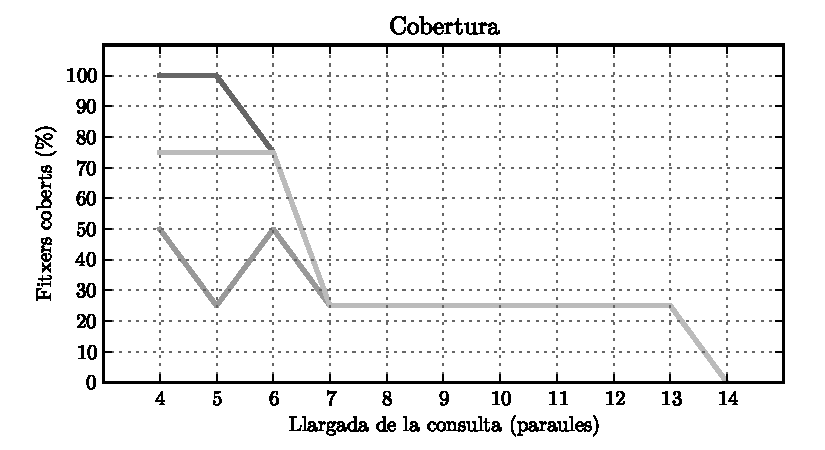
\includegraphics[width=0.8\textwidth]{figures/results:pageheader-reslen.pdf}
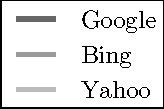
\includegraphics[scale=0.8]{figures/results:search-legend.pdf}
\caption{Qualitat dels resultats per fitxers amb una p�gina sencera com a cap�alera}
\label{fig:results:pageheader-reslen}
\end{center}
\end{figure}

Veiem que per aquest tipus d'article, el percentatge de p�gines per les quals s'han obtingut bons resultats disminueix molt a mesura que s'augmenta la llargada de la consulta. Cal tenir en compte que les consultes s'han obtingut totes a partir de la primera p�gina del fitxer. Al no contenir el resum, fa que l'expressi� regular usada per trobar la consulta no tingui coincid�ncies per la majoria dels articles provats. Si executem les mateixes proves, per� agafant les consultes de les dues primeres p�gines, els resultats milloren for�a:

\begin{figure}[H]
\begin{center}
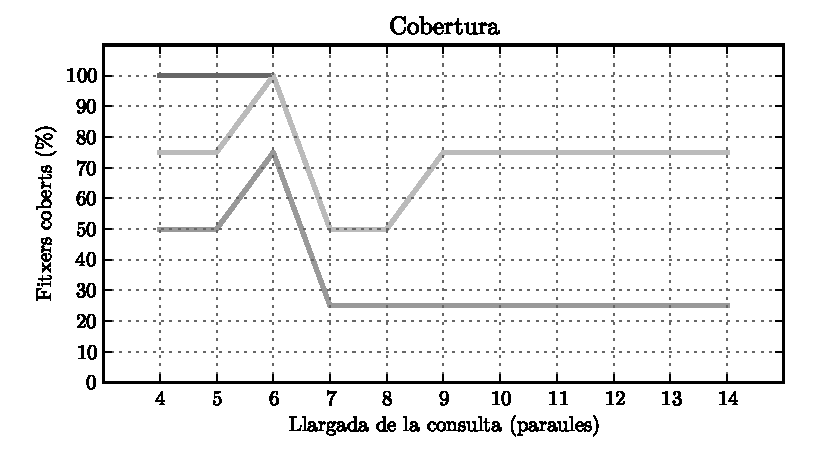
\includegraphics[width=0.8\textwidth]{figures/results:pageheader2-reslen.pdf}
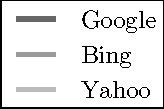
\includegraphics[scale=0.8]{figures/results:search-legend.pdf}
\caption{Qualitat dels resultats per fitxers amb una p�gina sencera com a cap�alera II}
\label{fig:results:pageheader2-reslen}
\end{center}
\end{figure}

El gr�fic de la figura seg�ent s'ha obtingut a partir d'articles que tenen una cap�alera \textit{normal}. Considerem que les cap�aleres dels articles m�s habituals s�n aquelles que tenen l'\textit{abstract} a la mateixa p�gina.
\begin{figure}[H]
\begin{center}
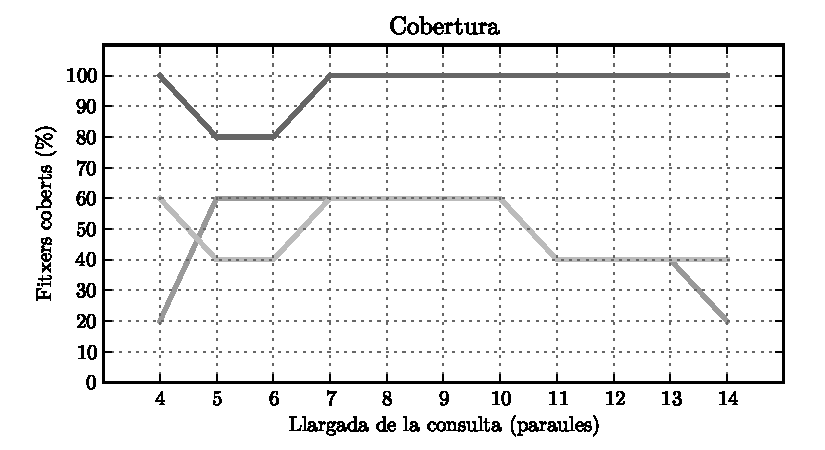
\includegraphics[width=0.8\textwidth]{figures/results:usualheader-reslen.pdf}
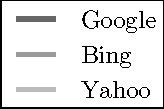
\includegraphics[scale=0.8]{figures/results:search-legend.pdf}
\caption{Qualitat dels resultats per fitxers amb cap�aleres \textit{normals}}
\label{fig:results:usualheader-reslen}
\end{center}
\end{figure}

\paragraph{}
Pel que fa al n�mero de consultes necess�ries per comen�ar a obtenir bons resultats, els gr�fics per aquests dos conjunts de fitxers s�n molt semblants al que hem vist a la figura \ref{fig:results:random-fqlen}.

\section{Generaci� de \textit{wrappers}}
\label{appendix:results:section:wrapperinduction}
Pel que fa a la generaci� autom�tica de regles d'extracci�, la figura seg�ent mostra els \textit{wrappers} obtinguts al generar-los fent servir nom�s dos exemples. Com es pot comprovar,
A continuaci� es mostren els gr�fics de la cobertura dels \textit{wrappers} generats per altres camps que no s'han tractat a la secci� \ref{chapter:results:section:wrapperinduction}.


\begin{figure}[H]
\begin{center}
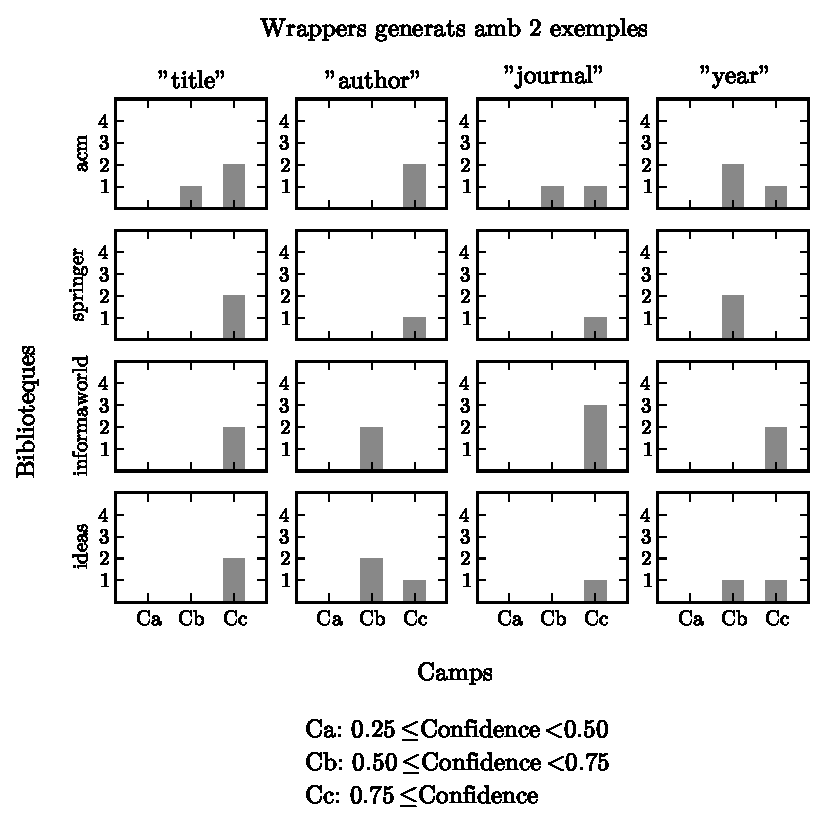
\includegraphics[width=0.8\textwidth]{figures/results:nwrappers-2.pdf}
\caption{Nombre de \textit{Wrappers} generats utilitzant 2 exemples i agrupats per confian�a}
\label{fig:results:nwrappers-2}
\end{center}
\end{figure}


\begin{figure}[H]
\begin{center}
\begin{minipage}{0.49\linewidth}
	\centering
	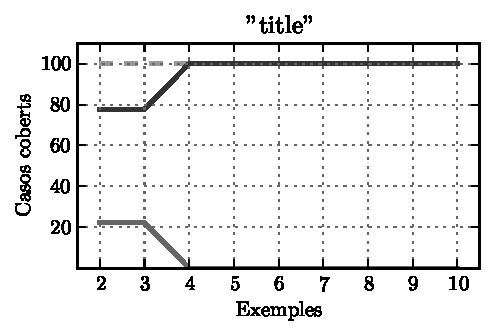
\includegraphics[width=\textwidth]{figures/results:coverage-title.pdf}
\end{minipage}
\hspace{0cm}
\begin{minipage}{0.49\linewidth}
	\centering
	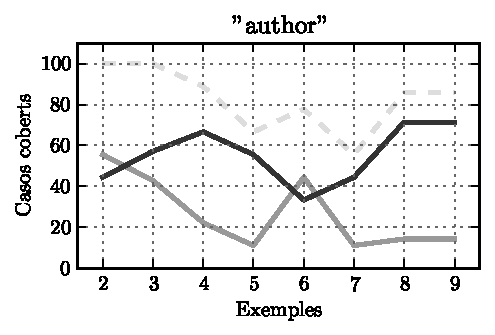
\includegraphics[width=\textwidth]{figures/results:coverage-author.pdf}
\end{minipage}
\end{center}
\end{figure}

\begin{figure}[H]
\begin{center}
\begin{minipage}{0.49\linewidth}
	\centering
	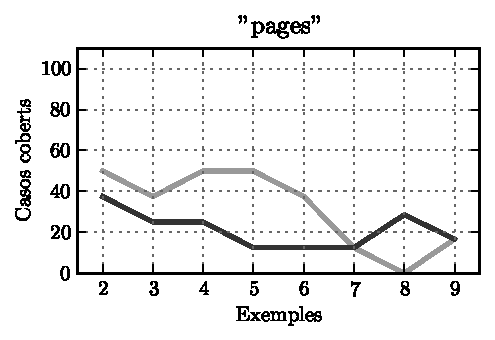
\includegraphics[width=\textwidth]{figures/results:coverage-pages.pdf}
\end{minipage}
\hspace{0cm}
\begin{minipage}{0.49\linewidth}
	\centering
	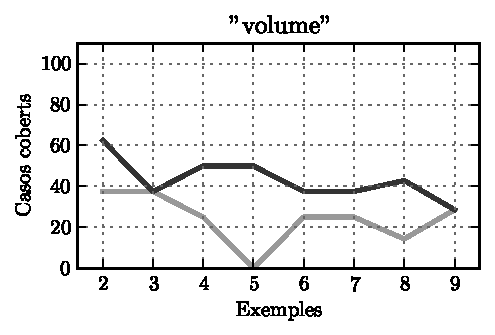
\includegraphics[width=\textwidth]{figures/results:coverage-volume.pdf}
\end{minipage}

\begin{minipage}{\linewidth}
	\centering
	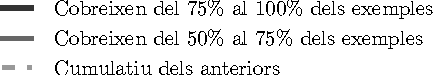
\includegraphics{figures/results:coverage-legend.pdf}
\end{minipage}

\caption{Cobertura dels \textit{wrappers} generats}
\label{fig:appendix:results:wrapperinduction:coverage}
\end{center}
\end{figure}



\begin{figure}[H]
\begin{center}
	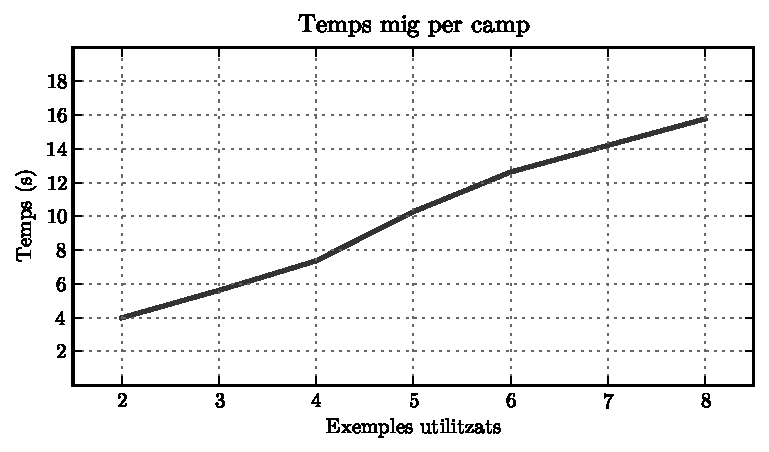
\includegraphics[width=0.8\textwidth]{figures/results:field-time.pdf}
	\caption{Temps mitj� per la generaci� dels \textit{wrappers} d'un �nic camp}
	\label{fig:appendix:results:wrapperinduction:time}
\end{center}
\end{figure}
	



\chapter{Diagrames}
\label{appendix:diagrams}
En aquest ap�ndix es mostren alguns diagrames que poden ajudar a entendre una mica millor l'aplicaci�. Creiem que cada diagrama �s auto-explicatiu nom�s s'acompanyen d'una petita descripci� als peus de cadascun d'ells.

\begin{figure}[H]
\begin{center}
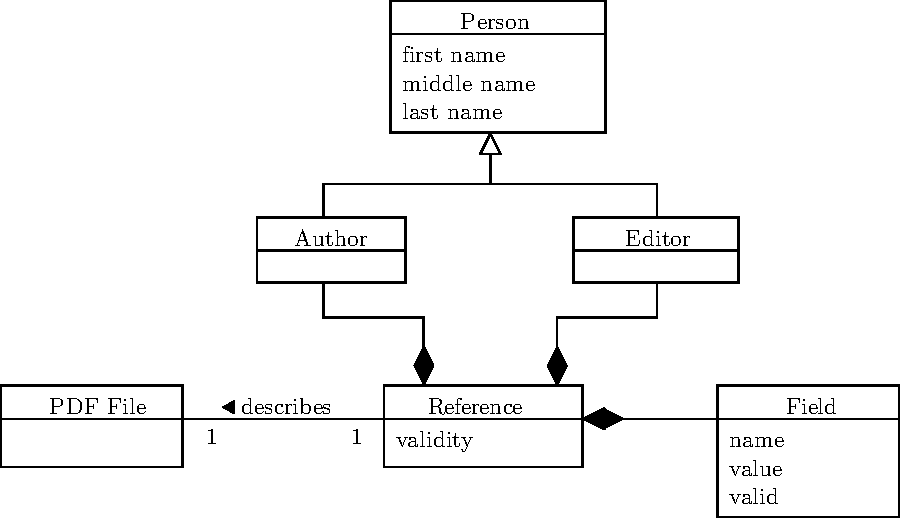
\includegraphics[width=0.7\textwidth]{figures/diagrams:references-domain-model.pdf}
\caption{Model de domini respecte les refer�ncies}
\label{fig:diagrams:references-domain-model}
\end{center}
\end{figure}


\begin{figure}[H]
\begin{center}
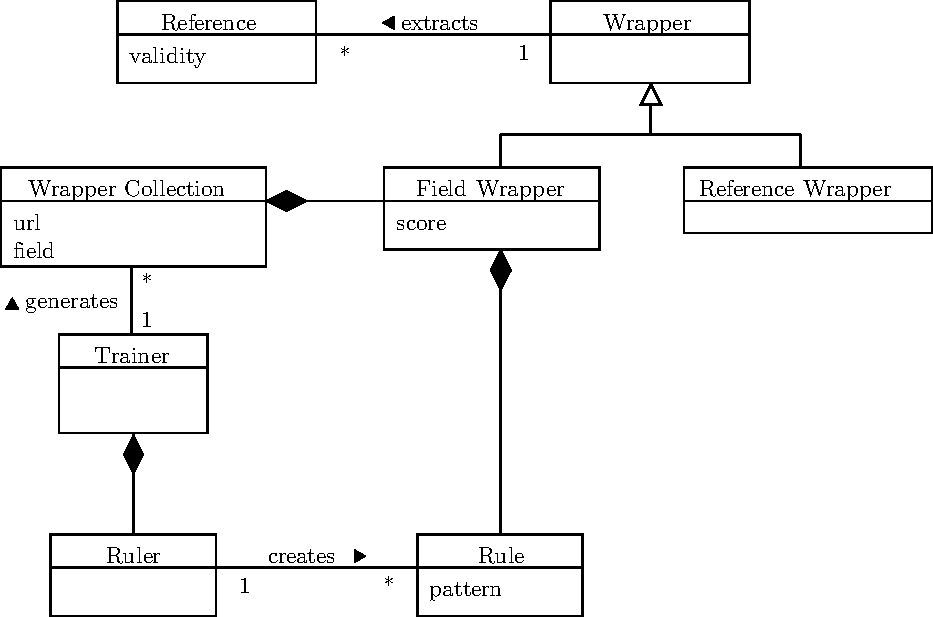
\includegraphics[width=0.7\textwidth]{figures/diagrams:wrappers-domain-model.pdf}
\caption{Model de domini dels \textit{wrappers}}
\label{fig:diagrams:wrappers-domain-model}
\end{center}
\end{figure}

\begin{figure}[H]
\begin{center}
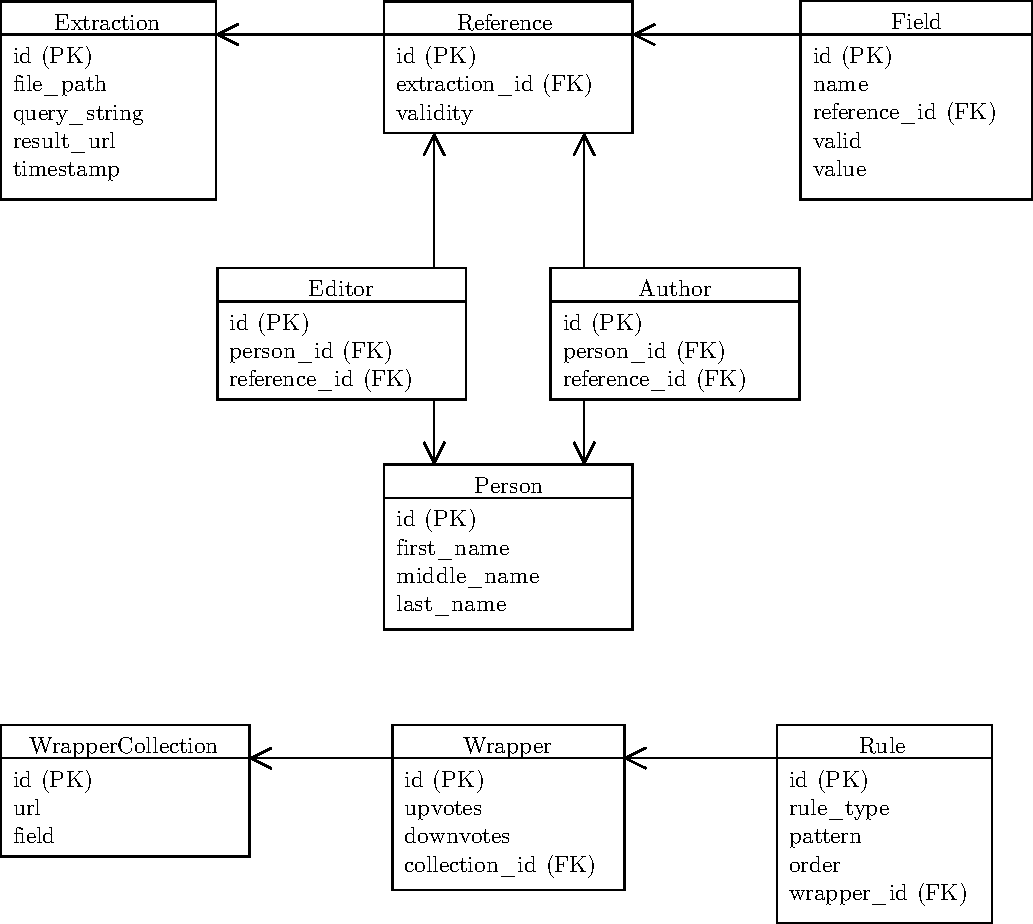
\includegraphics[width=0.8\textwidth]{figures/diagrams:database-diagram.pdf}
\caption{Estructura de la base de dades}
\label{fig:diagrams:database-diagram}
\end{center}
\end{figure}


\begin{figure}[ht]
\begin{center}
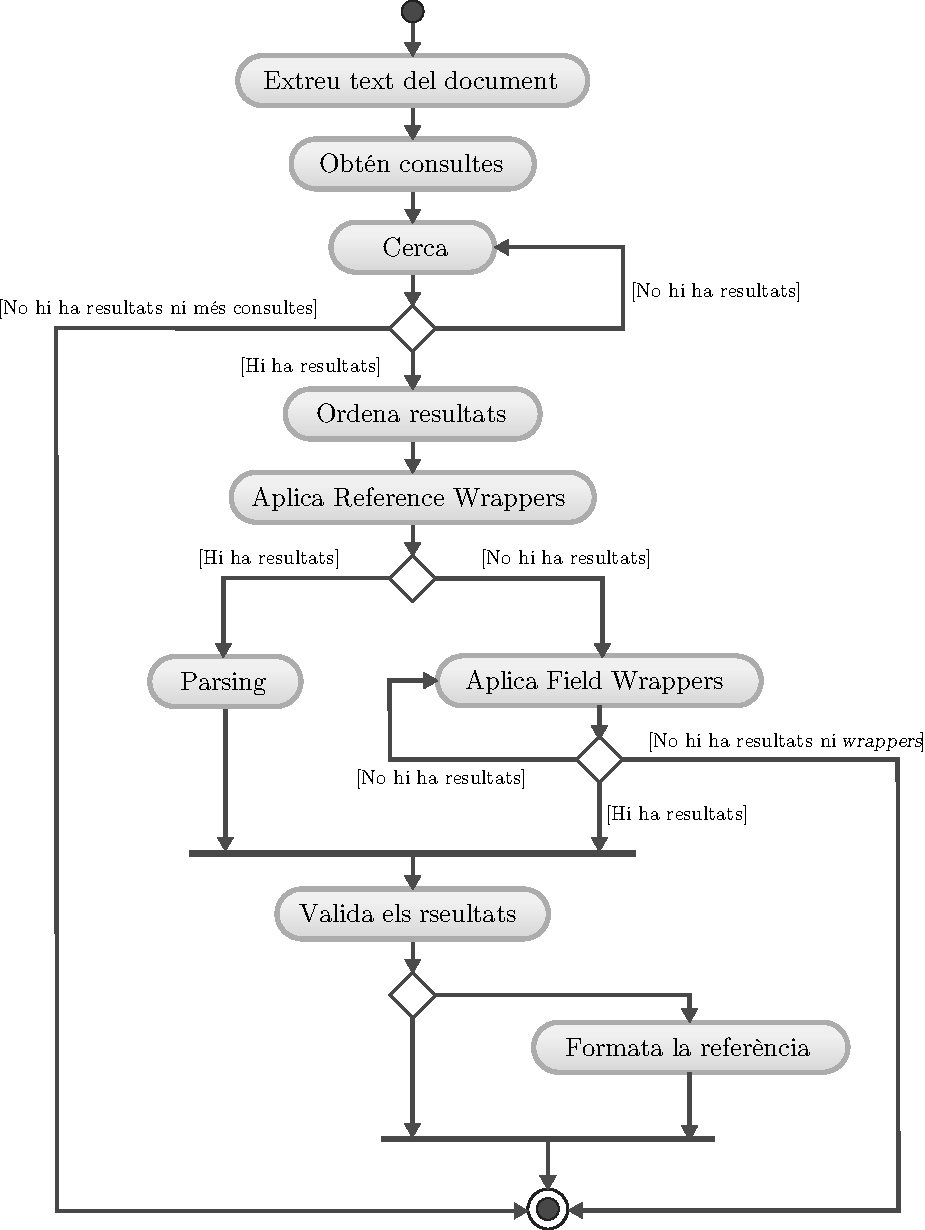
\includegraphics[width=0.95\textwidth]{figures/diagrams:extraction-activity.pdf}
\caption{Diagrama d'activitat per l'extracci� de refer�ncies}
\label{fig:diagrams:extraction-activity}
\end{center}
\end{figure}

\clearpage





\chapter{Extracci� Contingut PDF}
\label{appendix-pdf2text}

A continuaci� es mostren exemples de com queden les cap�aleres d'alguns fitxers PDF a l'extreure-les en forma de text.

\section{Exemple 01}
\subsubsection{Estructura del PDF}
\begin{figure}[H]
\begin{center}

\includegraphics[width=0.85\textwidth]{figures/pdf2text/pdf2text:01.pdf}
%\caption{Primera idea per l'extracci� de refer�ncies}
\label{fig:pdf2text:01}
\end{center}
\end{figure}

\subsubsection{Text}
Discrete Applied Mathematics 147 (2005) 43 � 55 www.elsevier.com/locate/dam

Pseudo-models and propositional Horn inference
Bernhard Ganter , R�diger Krau�e
Institut f�r Algebra, Technische Universit�t Dresden, Zellescher Weg 12-14, D-01062 Dresden, Germany Received 4 May 2001; received in revised form 6 January 2003; accepted 21 June 2004 Available online 29 December 2004

Abstract A well-known result is that the inference problem for propositional Horn formulae can be solved in linear time. We show that this remains true even in the presence of arbitrary (static) propositional background knowledge. Our main tool is the notion of a cumulated clause, a slight generalization of the usual clauses in Propositional Logic. We show that each propositional theory has a canonical irredundant base of cumulated clauses, and present an algorithm to compute this base. � 2004 Elsevier B.V. All rights reserved.
MSC: 03B05; 03B35; 68T30 Keywords: Horn inference; Horn base; Background knowledge


\section{Exemple 02}
\subsubsection{Estructura del PDF}
\begin{figure}[H]
\begin{center}
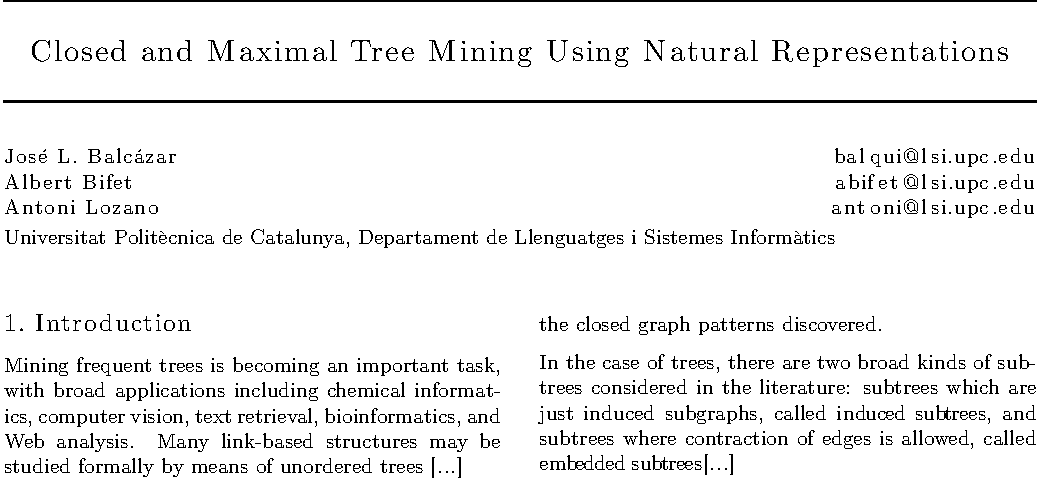
\includegraphics[width=0.85\textwidth]{figures/pdf2text/pdf2text:02.pdf}
\label{fig:pdf2text:02}
\end{center}
\end{figure}

\subsubsection{Text}
Closed and Maximal Tree Mining Using Natural Representations

Jos' L. Balc'zar e a balqui@lsi.upc.edu Albert Bifet abifet@lsi.upc.edu Antoni Lozano antoni@lsi.upc.edu Universitat Polit`cnica de Catalunya, Departament de Llenguatges i Sistemes Inform`tics e a

1. Introduction
Mining frequent trees is becoming an important task, with broad applications including chemical informatics, computer vision, text retrieval, bioinformatics, and Web analysis. Many link-based structures may be studied formally by means of unordered trees.


\section{Exemple 03}
\subsubsection{Estructura del PDF}
\begin{figure}[H]
\begin{center}

\includegraphics[width=0.85\textwidth]{figures/pdf2text/pdf2text:03.pdf}
\label{fig:pdf2text:03}
\end{center}
\end{figure}

\subsubsection{Text}
Applied Economics, 2010, 42, 825�850
\\
\\
Modelling the interactions across international stock, bond and foreign exchange markets\\
Abdul Hakima,* and Michael McAleerb\\
Department of Economics, University of Western Australia, Australia and Faculty of Economics, Indonesian Islamic University, Indonesia b Department of Economics, University of Western Australia, Australia
a
\\
\\
Downloaded By: [Consorci de Biblioteques Universitaries de Catalunya] At: 11:49 20 May 2010\\
\\
The benefits of investing internationally depend on three conditions, namely, cross-country correlations, market volatilities and future changes in currency risks (Odier and Solnik, 1993). This article investigates these conditions for several countries. Many papers have modelled [...]

\chapter{Manual d'usuari}

L'aplicaci� es distribueix en forma d'\texttt{egg} de \textit{Python} i pot ser instal�lada de la manera est�ndard amb la comanda \texttt{easy\_install} (m�s detalls a \cite{pyEasyInstall}). Aquest cap�tol se centra a descriure alguns dels aspectes d'utilitzaci� de l'aplicaci� un cop instal�lada i mitjan�ant la interf�cie gr�fica. B�sicament, tindrem un men� amb dues grans categories: \textit{references} i \textit{wrappers}. Vegem qu� hi ha en cadascuna d'elles.

\section{Refer�ncies}

%%%% EXTRACT %%%%
\subsubsection{Extracci�}
La primera opci� del men� �s la que permet llegir un directori de fitxers PDF i obtenir-ne les refer�ncies. El sistema inclou \textit{wrappers} per les biblioteques digitals que s'han descrit en altres cap�tols d'aquest document, i per tant, des d'un principi ja es pot provar a fer extraccions d'articles indexats per aquestes biblioteques.
\\
\\
La vista de la figura \ref{fig:screenshots:extract-references} mostra el camp �nic que cal omplir per tal de comen�ar l'extracci�: simplement seleccionem un directori o fitxer i cliquem el bot� \textit{Extract References}. Durant l'execuci�, es mostra una barra de progr�s i una vegada finalitzat, se'ns mostrar� una finestra molt semblant a la de la figura \ref{fig:screenshots:import-references-2} indicant-nos que podem veure i editar les refer�nceies amb l'opci� del men� \textit{Manage}.
\begin{figure}[ht]
\begin{center}
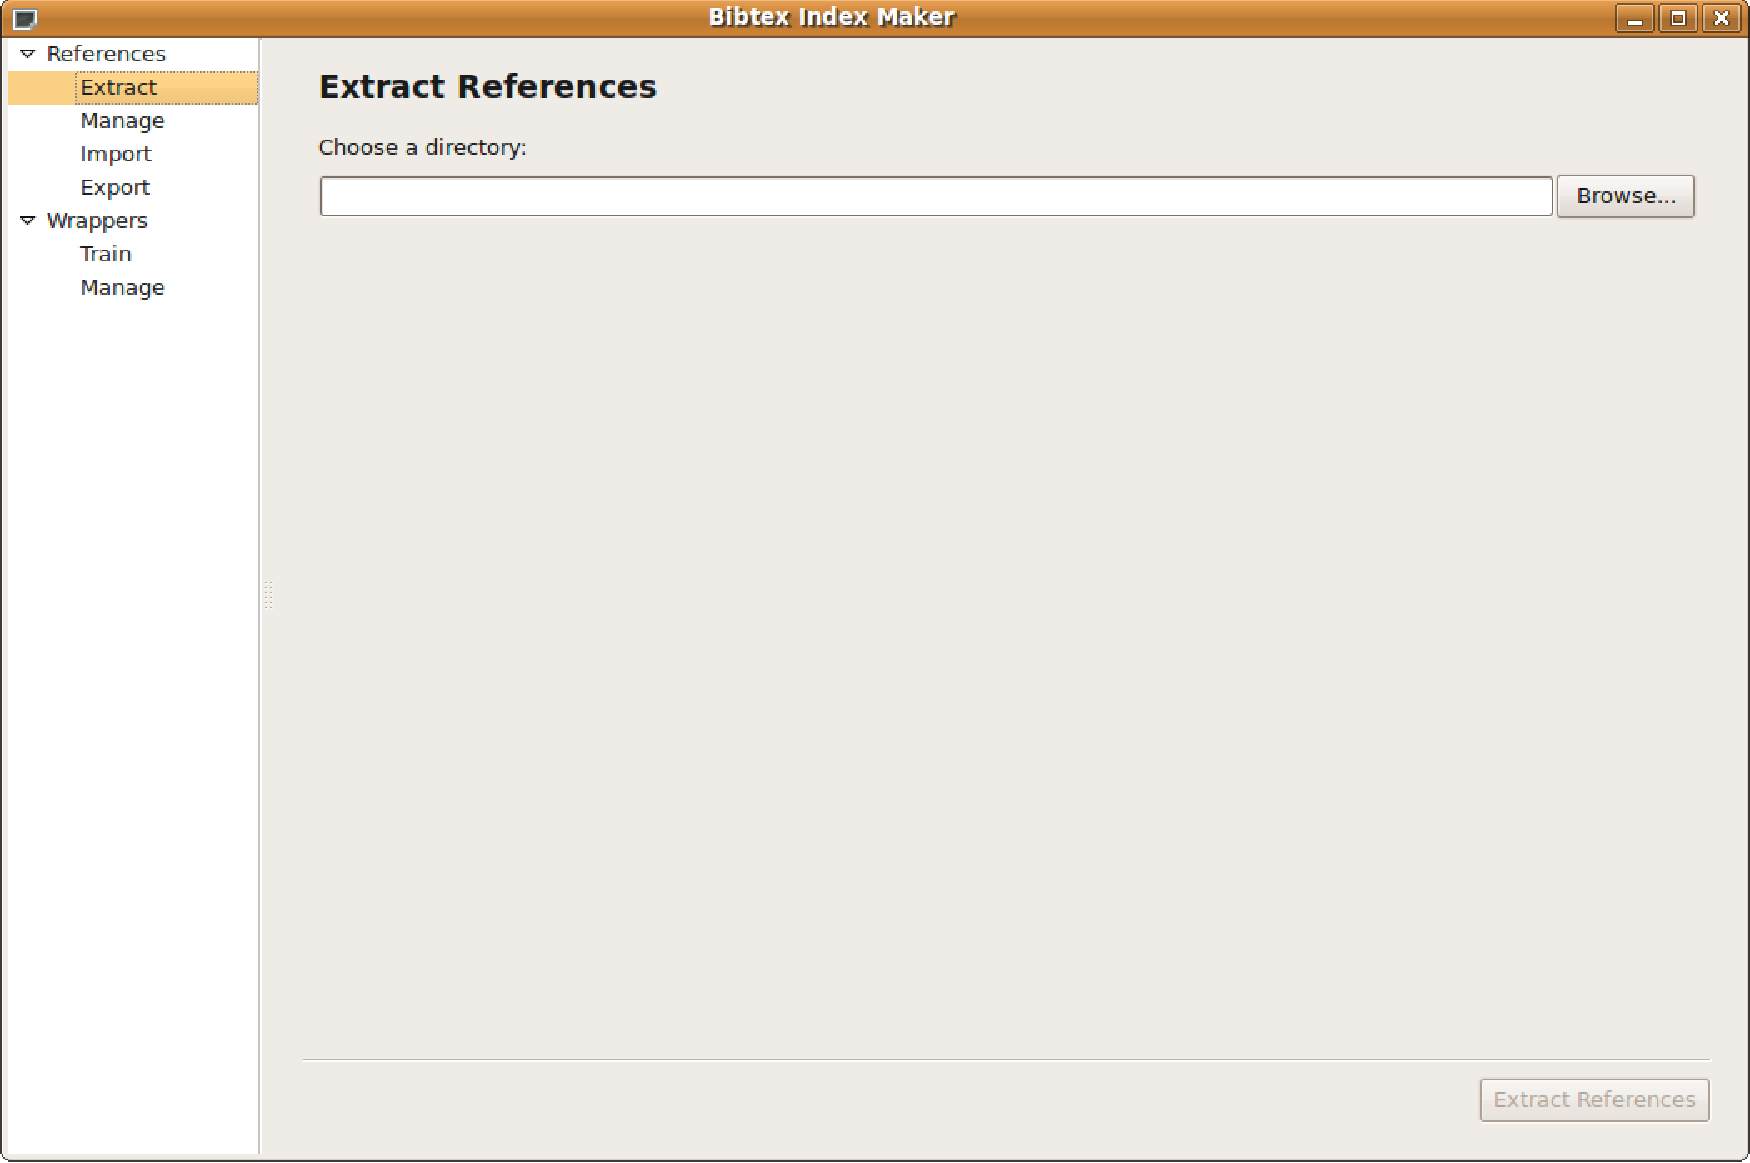
\includegraphics[width=0.9\textwidth]{figures/screenshots/screenshots:extract-references.pdf}
\caption{Extreu refer�ncies}
\label{fig:screenshots:extract-references}
\end{center}
\end{figure}

%%%% MANAGE %%%%
\subsubsection{Gesti�}
Amb l'opci� \textit{Manage} (veure \ref{fig:screenshots:manage-references}) podrem gestionar les refer�ncies disponibles i realitzar les operacions CRUD t�piques. A la part esquerra es mostra un llistat de totes les refer�ncies de la base de dades. Al seleccionar-ne una s'omplir� l'editor de la meitat dreta de la finestra amb tota la informaci� sobre la refer�ncia.

\begin{figure}[ht]
\begin{center}
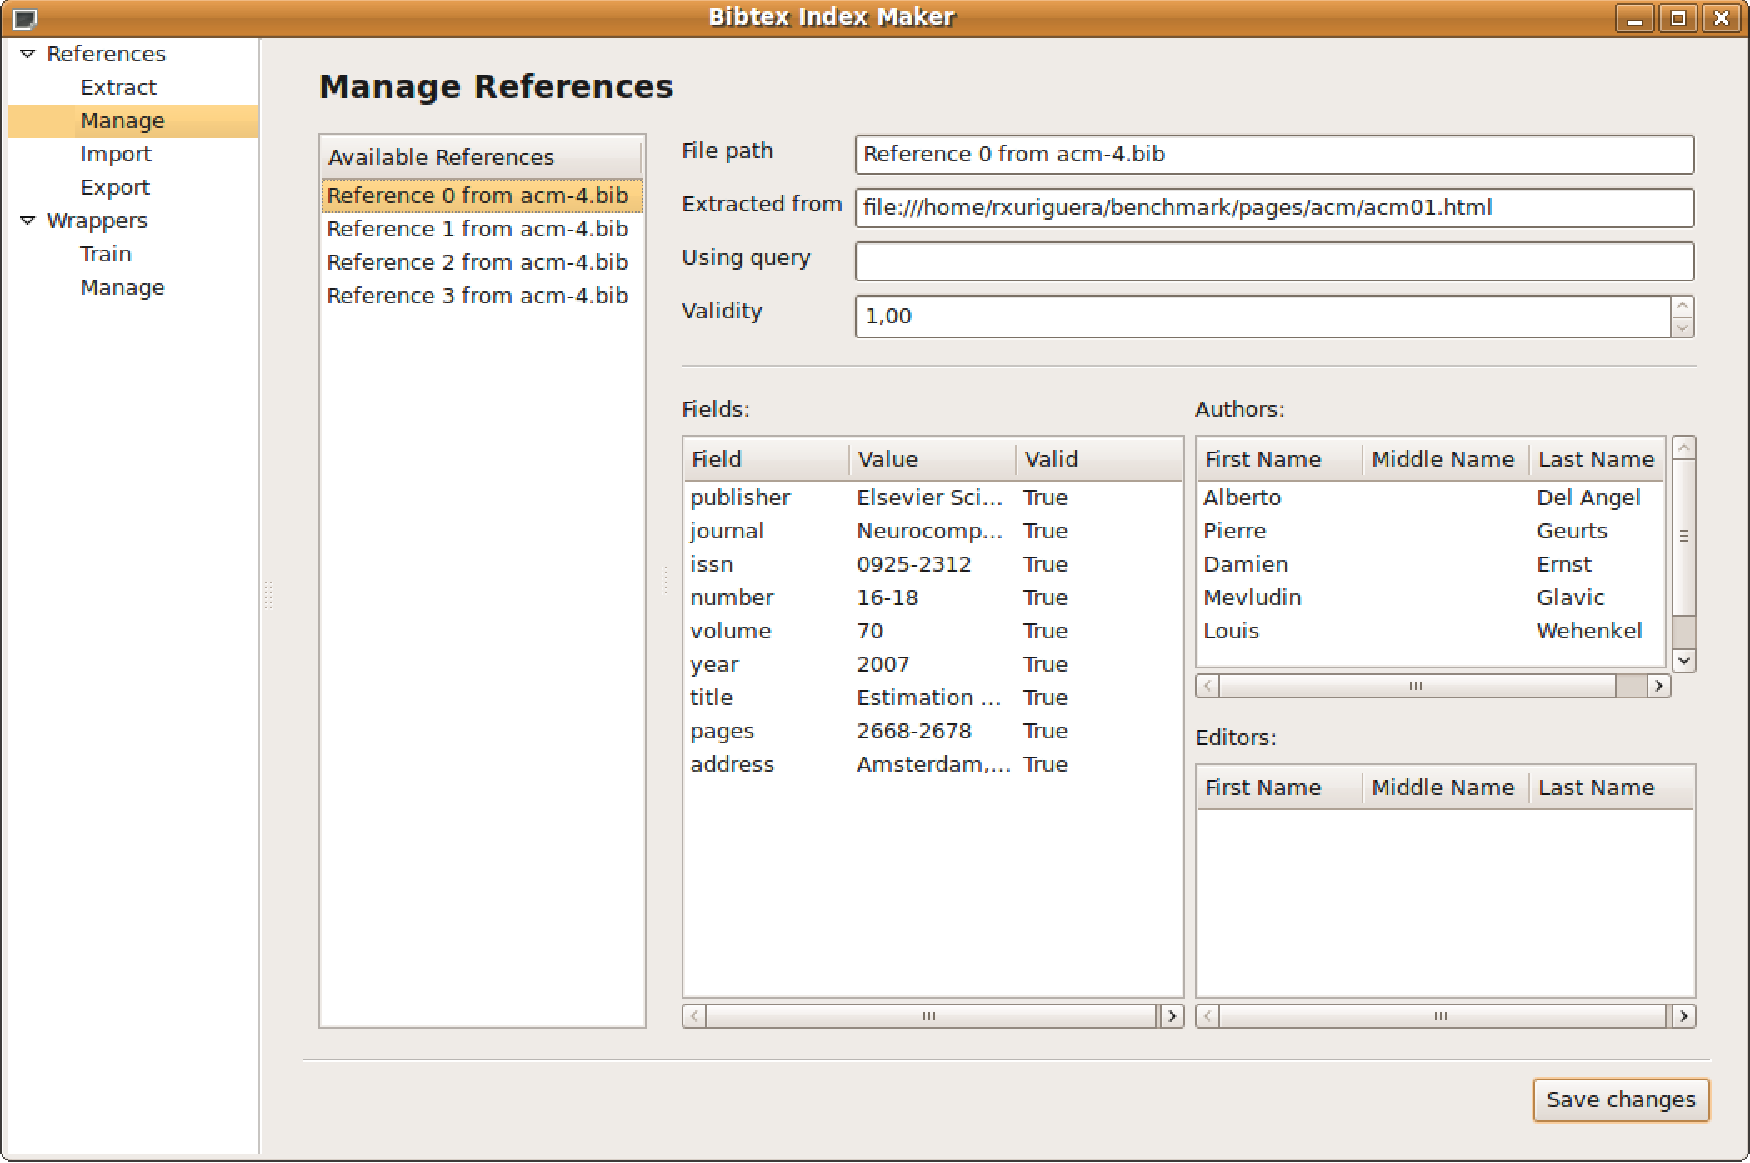
\includegraphics[width=0.9\textwidth]{figures/screenshots/screenshots:manage-references.pdf}
\caption{Maneig de refer�ncies}
\label{fig:screenshots:manage-references}
\end{center}
\end{figure}

Algunes caracter�stiques:
\begin{itemize}
\item{}
Podem crear nous camps, autors i editors simplement afegint-los al final de la llista adequada, a la l�nia buida que hi ha. Per eliminar-los, nom�s cal esborrar totes les columnes i deixar la fila en blanc.
\item{}
Per afegir o eliminar noves refer�ncies podem fer-ho a partir del men� contextual que apareix al clicar amb el bot� secundari sobre la llista \textit{Available References}.
\item{}
�s necessari definir una URL com a valor del camp \textit{Extracted from} si posteriorment es pret�n utilitzar la refer�ncia en q�esti� per generar \textit{wrappers}.
\item{}
Pel que fa al camp \textit{File Path}, nom�s serveix per ajudar a l'usuari a distingir entre les m�ltiples refer�ncies disponibles de la llista \textit{Available References}.
\end{itemize}

%%%% IMPORT %%%%
\subsubsection{Importaci�}
\begin{figure}[ht]
\begin{center}
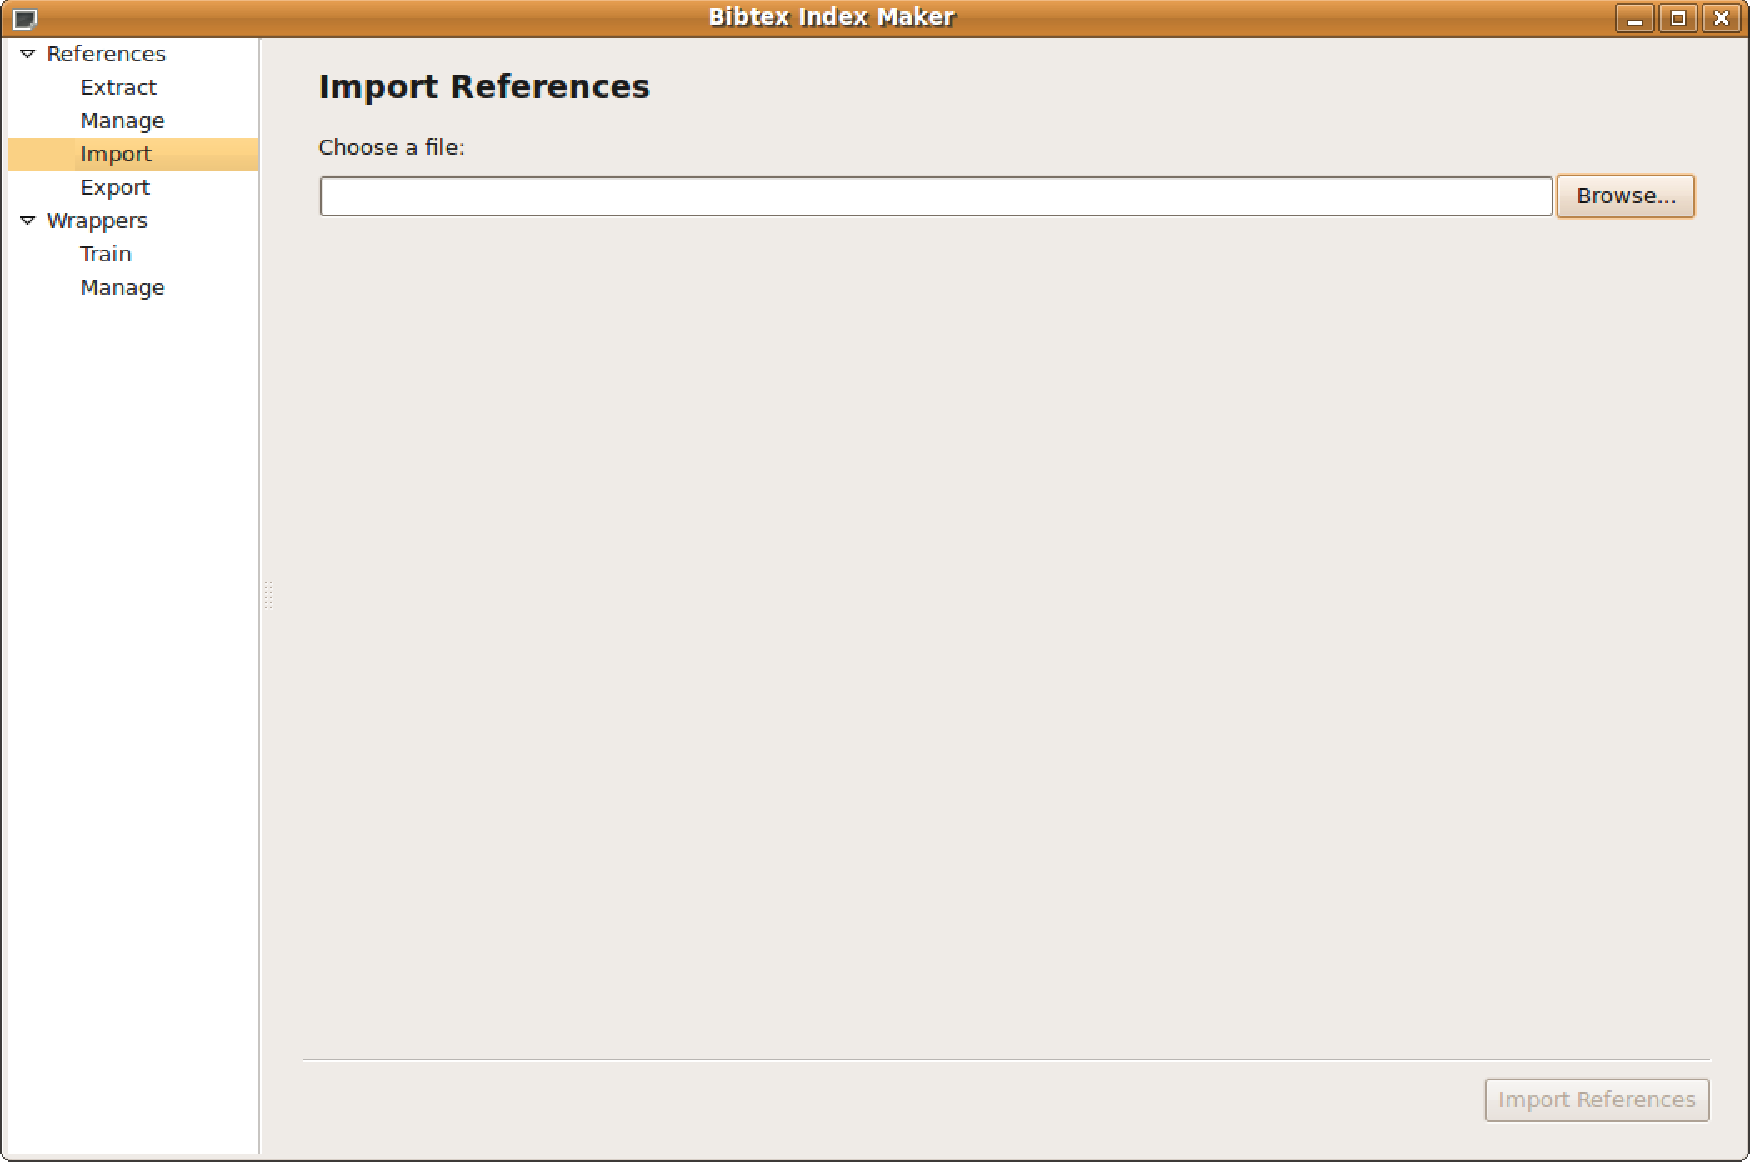
\includegraphics[width=0.9\textwidth]{figures/screenshots/screenshots:import-references.pdf}
\caption{Importa refer�ncies}
\label{fig:screenshots:import-references}
\end{center}
\end{figure}
Aquesta opci� �s la que probablement m�s ens interessar� la primera vegada que executem l'aplicaci� just despr�s d'instal�larla. Permet importar refer�ncies des de fitxers \texttt{.bib} de manera que sigui ben f�cil comen�ar a generar \textit{wrappers} i configurar el sistema segons les necessitats de cadasc�. El funcionament �s molt semblant al de les extraccions. Se selecciona un fitxer a la finestra \ref{fig:screenshots:import-references} i un cop s'ha acabat, se'ns redirigir� a la vista de la figura \ref{fig:screenshots:import-references-2}.


\begin{figure}[ht]
\begin{center}
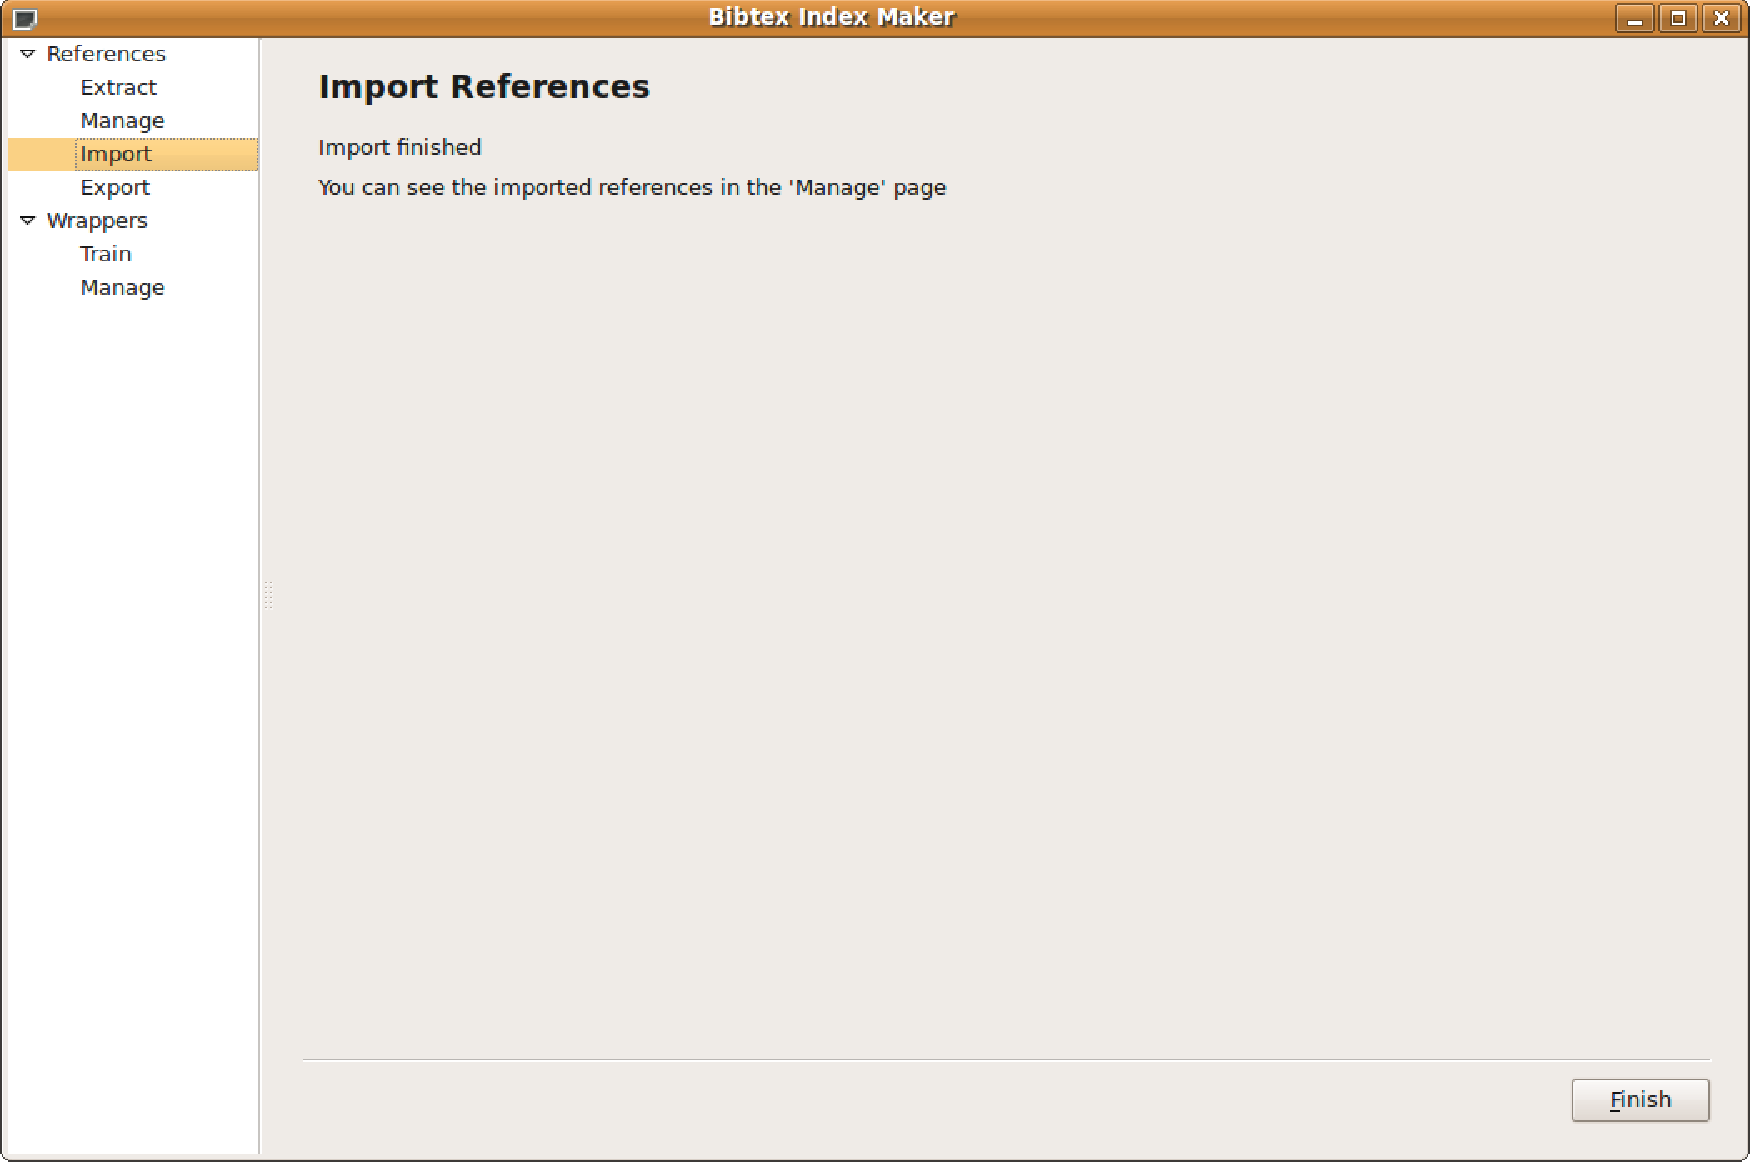
\includegraphics[width=0.9\textwidth]{figures/screenshots/screenshots:import-references-2.pdf}
\caption{Un cop s'han importat les refer�ncies}
\label{fig:screenshots:import-references-2}
\end{center}
\end{figure}

%%%% EXPORT %%%%
\subsubsection{Exportaci�}
La darrera opci� que queda relacionada amb les refer�ncies �s la funcionalitat que permet exportar-les en format \BibTeX{}. De la mateixa manera que amb la finestra \textit{Manage}, a la part esquerra se'ns lllistaran totes les refer�ncies disponibles. Podrem seleccionar les que vulguem i la seva entrada formatada apareixer� a l'�rea de text de la part dreta. Hi ha la possibilitat de seleccionar o b� desseleccionar tots els elements de la llista a partir del men� contextual que apareix al fer clic amb el bot� secundari.
Tamb� podem desar totes les entrades seleccionades directament a un fitxer amb el bot� \textit{Save to file}.

\begin{figure}[ht]
\begin{center}
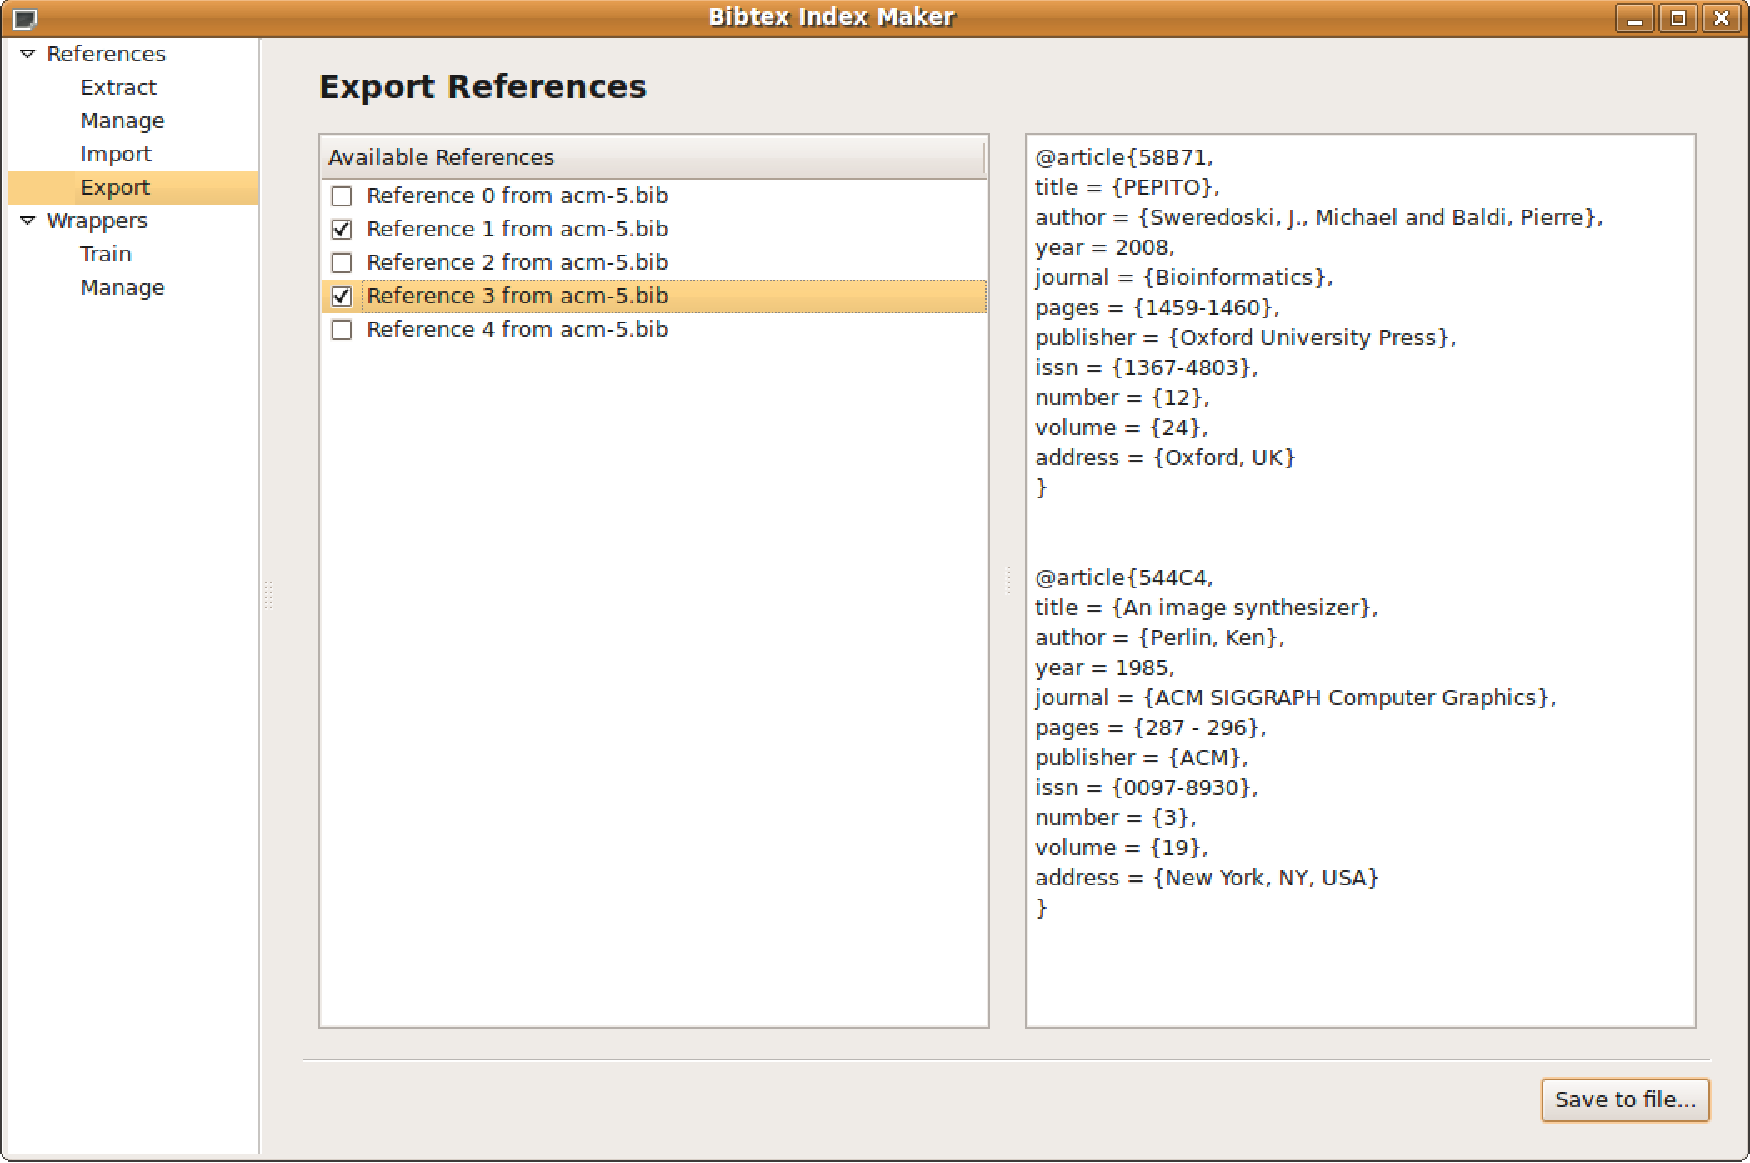
\includegraphics[width=0.9\textwidth]{figures/screenshots/screenshots:export-references.pdf}
\caption{Exporta refer�ncies}
\label{fig:screenshots:export-references}
\end{center}
\end{figure}


%%%% WRAPPERS %%%%
\clearpage
\section{\textit{Wrappers}}
L'altra categoria �s la que permet gestionar els \textit{wrappers}. 


%%%% TRAIN %%%%
\subsubsection{Entrenament}
Aquesta opci� �s la que ens permet generar nous \textit{wrappers} a partir de les refer�ncies de les que es disposa. La vista que permet executar aquesta funcionalitat �s la de la figura \ref{fig:screenshots:wrapper-train}. Les URLs de les biblioteques per les quals ja s'han generat \textit{wrappers} amb anterioritat es mostren a la llista \textit{Available URLs}, facilitant el re-entrenament un cop les dades deixen d'extreure's correctament. En el cas que es tracti d'una biblioteca nova, podem introduir-ne la seva adre�a (o un prefix) manualment al camp \textit{URL}.
\\
\\
Un cop hem escollit la biblioteca, nom�s hem de clicar el bot� \textit{Train} i deixar que l'aplicaci� faci la resta. Quan finalitza, es mostra un missatge indicant que podem veure i editar els \textit{wrappers} generats des amb l'opci� \textit{Manage}.

\begin{figure}[ht]
\begin{center}
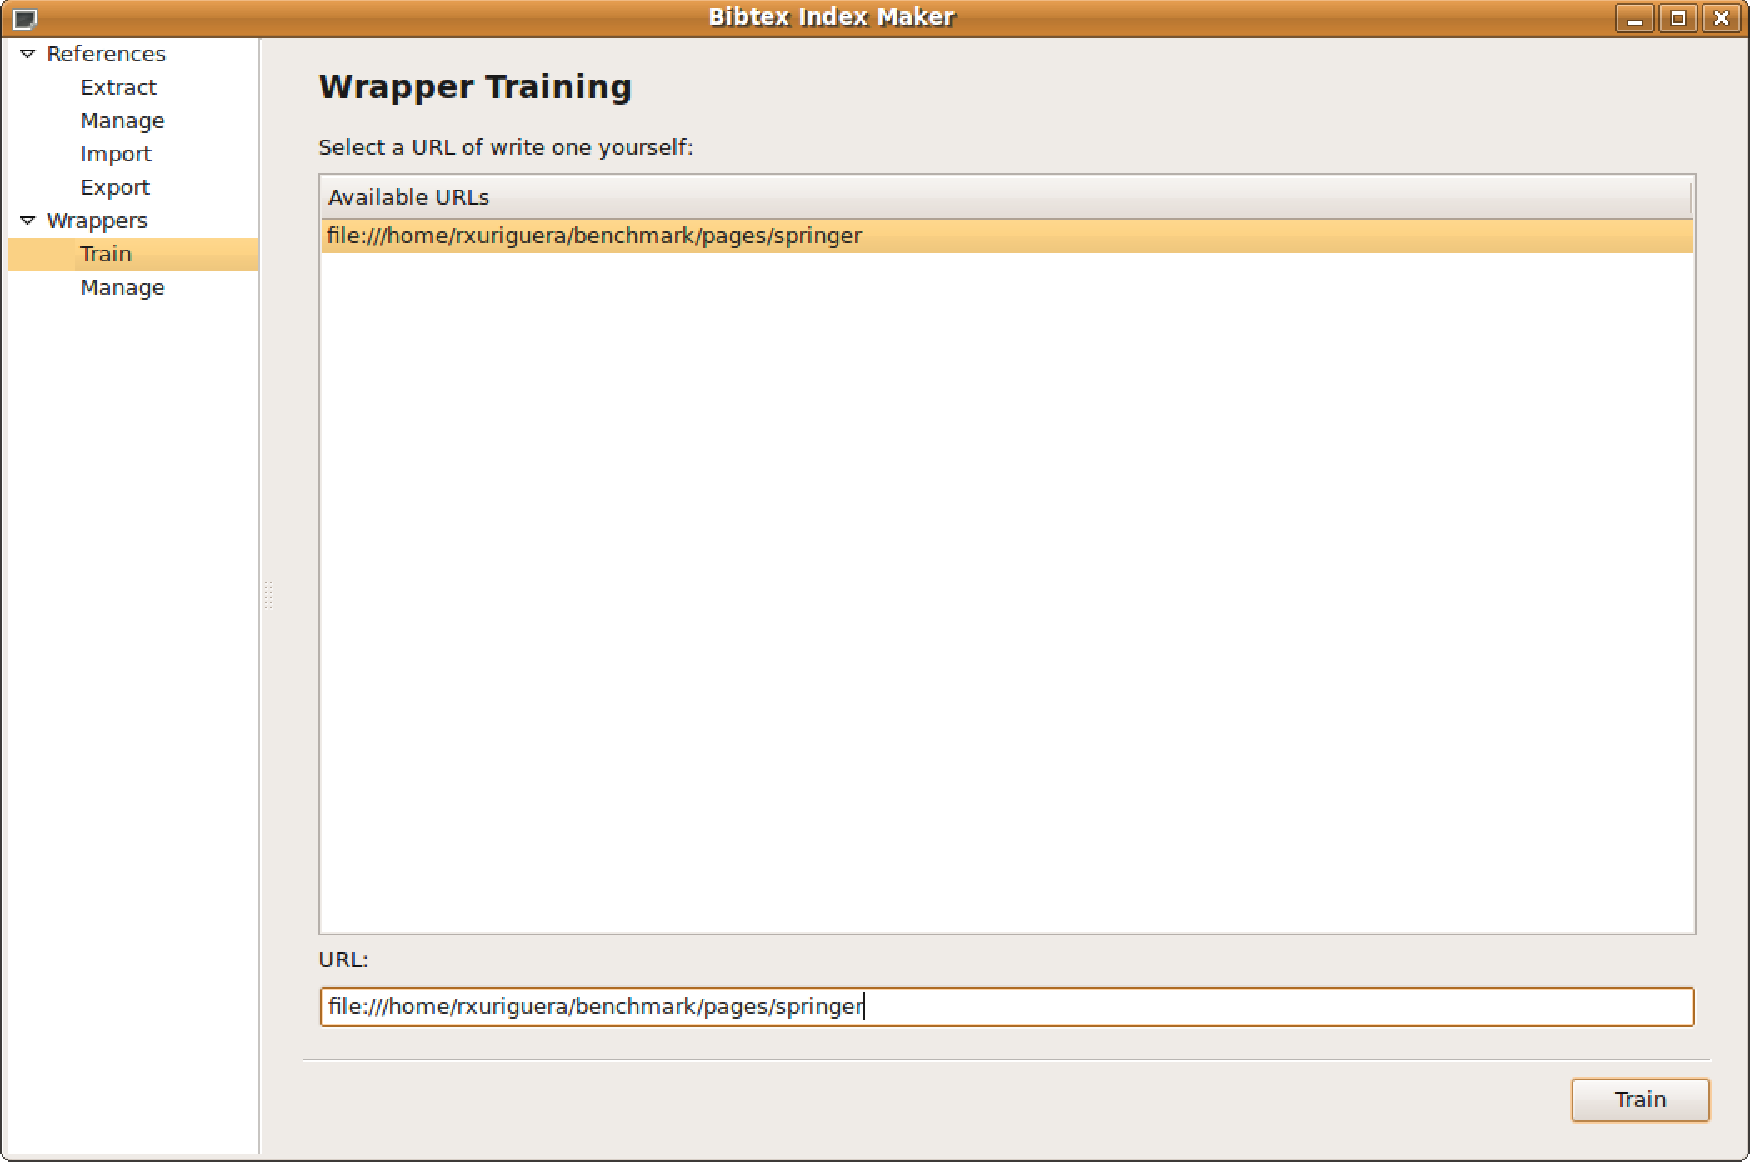
\includegraphics[width=0.9\textwidth]{figures/screenshots/screenshots:wrapper-train.pdf}
\caption{Entrenament de \textit{wrappers}}
\label{fig:screenshots:wrapper-train}
\end{center}
\end{figure}


%%%% MANAGE %%%%
\subsubsection{Gesti�}
De la mateixa manera que podem modificar les refer�ncies, tamb� tenim un editor pels \textit{wrappers} generats; es mostra a la finestra de la figura \ref{fig:screenshots:wrapper-manager}. En aquest cas tenim tres apartats:
\begin{itemize}
\item{}
Llistat de col�leccions de \textit{wrappers} agrupades segons la biblioteca digital a la qual corresponen.
\item{}
Llistat de \textit{wrappers} de la col�lecci� seleccionada en un moment donat. Per cadascun d'ells es mostra la puntuaci� rebuda.
\item{}
Editor del \textit{wrapper} seleccionat a la llista anterior. Es mostren els vots positius, negatius, la puntuaci� calculada i el llistat de regles.
\end{itemize}

Podem crear i eliminar regles afegint nous valors a la l�nia buida que hi ha al final de la llista \textit{Rules} i deixant l�nies en blanc, respectivament. Les col�leccions i els \textit{wrappers} es poden crear i esborrar amb el men� contextual que apareix al clicar amb el bot� secundari. Aquesta inconsist�ncia a l'hora de realitzar la mateixa operaci� per elements diferents �s un problema que caldr� solucionar en un futur.

\begin{figure}[ht]
\begin{center}
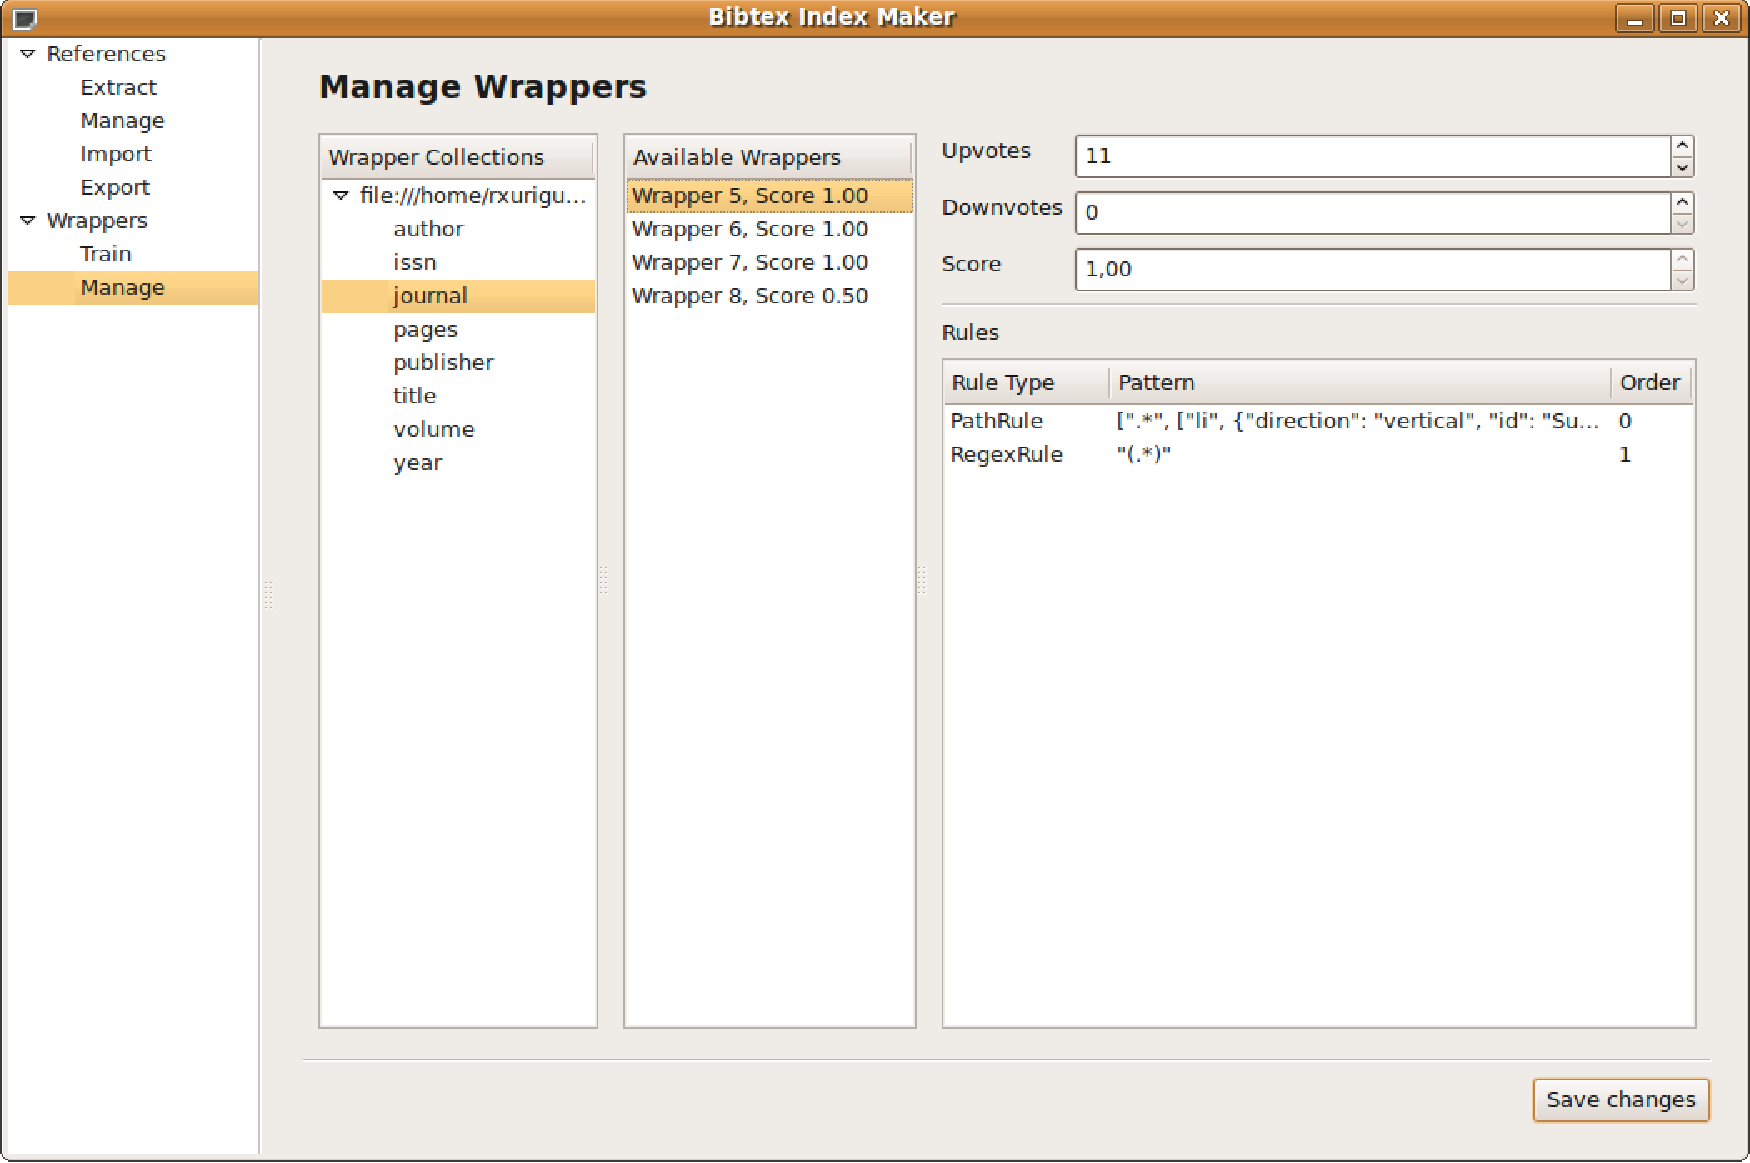
\includegraphics[width=0.9\textwidth]{figures/screenshots/screenshots:wrapper-manager.pdf}
\caption{Gesti� de \textit{wrappers}}
\label{fig:screenshots:wrapper-manager}
\end{center}
\end{figure}






\newpage
\thispagestyle{empty}
\mbox{}

\newpage
\thispagestyle{empty}
\mbox{}

\newpage
\thispagestyle{empty}
\mbox{}

\newpage
\thispagestyle{empty}
\mbox{}

\end{document}
